\documentclass[a4paper,12pt]{scrartcl}
\usepackage[utf8]{inputenc}
\usepackage{graphicx}
\usepackage{mathtools}
\usepackage{amsfonts}
\usepackage{gnuplottex}
\usepackage{fullpage}
\usepackage{wrapfig}
\usepackage{hyperref}
\usepackage{url}

% \setcounter{secnumdepth}{3}

\DeclareMathOperator*{\argmax}{arg\,max}
\DeclareMathOperator*{\argmin}{arg\,min}

\begin{document}

\titlehead{Université Libre de Bruxelles}
\title{Procedural City Generator Project}
\subtitle{INFO-H-502 - Image synthesis}
\author{Tim Lenertz}
\date{\today}
\maketitle

\section{Introduction}
The goal of this project is to develop a Blender add-on that generates a randomized city model. The city should consist of a street layout, different kinds of buildings, lakes, gardens and parcs. All of these elements should be randomized as well.

\section{Methodology}
In order to generate a credible model of a random city, a logical approach is to emulate the way a city evolves in reality: Streets are shaped according to the shape of the terrain, and in relation to previously existing infrastructure. Also the most developped part tends to be located near a city center, while more remote areas remain more rural.

This project is based on the \emph{Citygen} system described in \cite{Kell2007}. The city model is generated following these steps:
\begin{enumerate}
\item A terrain height-map is created featuring some erosion.
\item Primary streets are put on the terrain, and made to connect some randomly defined intersection points. The streets' shape is guided by the terrain shape.
\item The regions enclosed by primary streets are the \emph{city cells}. According to its distance from the center, each city cell is attributed a \emph{profile} that indicates whether this cell will contain a given type of city buildings and streets, or more rural content.
\item For city cells that shall contain city buildings, a network of \emph{secondary roads} is created. Starting from two or more points on the enclosing primary street cycle, secondry roads are \emph{grown} into the city cell using a recursive algorithm that simulates the real evolution of a street layout.
\item Each region enclosed by these secondary roads is called a \emph{block}. Each block is subdivided into \emph{lots}, and the lots placed next to a road will contain a building.
\item For each of these lots, a certain kind of building is created with some randomization.
\end{enumerate}
The following text describes these 6 steps in more detail. The problems encountered in implementing the algorithms are described in section \ref{sec:implementation}.

\subsection{Terrain}
For generating a random height map for the terrain, the \emph{diamond-square} algorithm is used. The basic idea is to start with a height map consisting only of a $2 \times 2$ matrix giving the elevations of the 4 corner points. A mid-point displacement algorithm then expands this into a $3 \times 3$ matrix by interpolating the 5 intermediate values and adding a random amount. Then the process is recursively repeated for each of the 4 new $2 \times 2$ submatrices, with a smaller random additive value. This process yields a fractal terrain height map, but with visual bias towards the X and Y directions of the grid, as can be seen in figure \ref{fig:plasma}

The diamond-square algorithm is an improvement which adds a ``diamond step'' after the ``square step'', so as to combine interpolation in the straight and diagonal directions. The roughness of the terrain can be parametrized. However a stongly uneven terrain causes problems with the algorithms, ad parts of the city (e.g. streets) will get under the terrain.

\begin{figure}[h]
\center
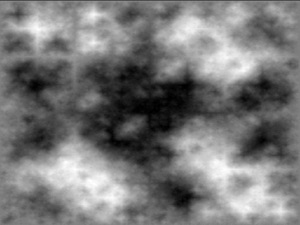
\includegraphics[width=10cm]{Plasmafractal.jpg}
\label{fig:plasma}
\caption{Result of mid-point displacement algorithm}
\end{figure}


\subsection{Primary Streets}
For the following steps, the procedure described in \cite{Kell2007} is used. The primary streets of the city are defined on two levels: a \emph{high-level} representation is a graph connecting the primary street junctions (intersection points). The \emph{low-level} representation describes the shape of the primary streets that interconnect the junction points. In order to get a more realistic output, they are not straight segments, but rather follow a curved path guided by the terrain.

The first step is to randomly create the high-level graph. It should randomly subdivide the terrain on the large scale such that the regions enclosed by primary street cycles not too small or too large. Different methods were attempted, such as to generate a Delaunay triangulation or a Voronoi diagram on a random point set. However these do not easily allow control over the shape and size of the resulting regions. Instead, the algorithm used is to begin with a regular grid, but then randomly displace the junction points by a normal distribution. The amount of deviation from a perfect grid can be parametrized. Figures \emph{fig:primaryS} and \emph{fig:primaryL} shows some examples of the primary street layout for different settings.

\begin{figure}[h]
\center
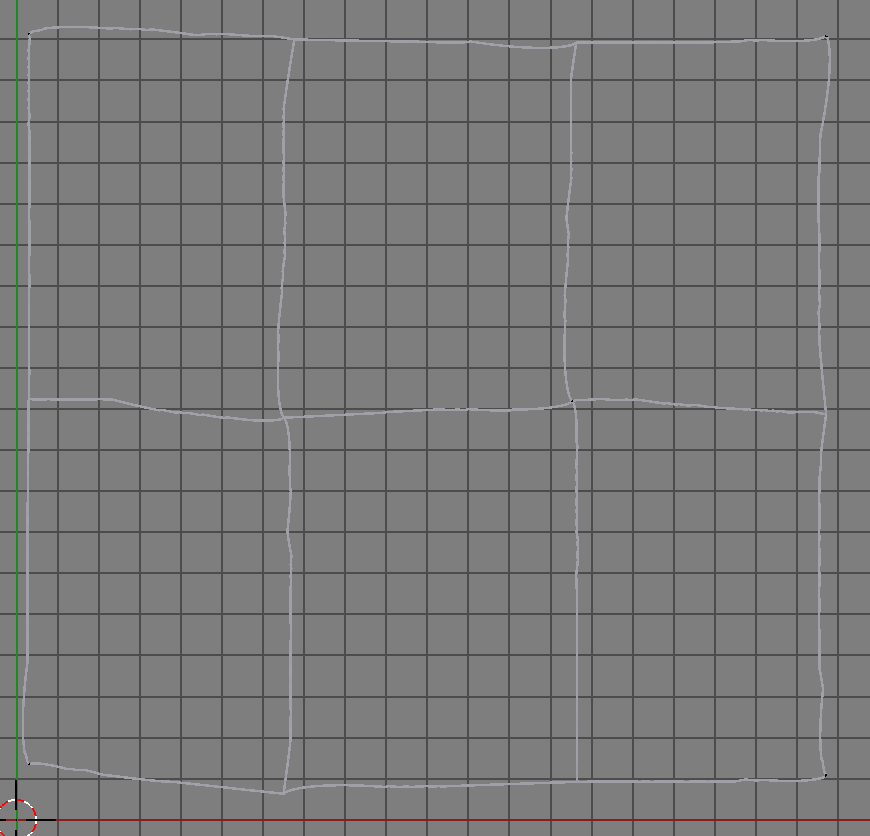
\includegraphics[width=10cm]{devS.png}
\caption{Primary streets with 6 intersection points and high grid alignment}
\label{fig:primaryS}
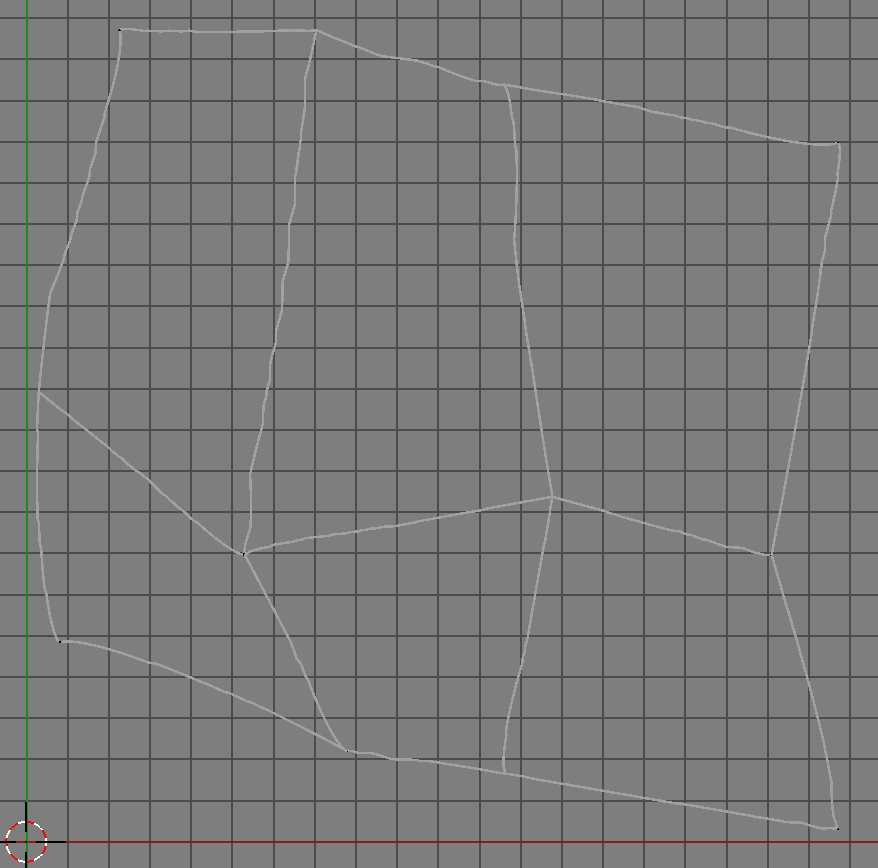
\includegraphics[width=10cm]{devL.png}
\caption{...low grid alignment}
\label{fig:primaryL}
\end{figure}

For the generation of the primary road shape, an iterative growth algorithm is used: In order to create the curved road from A to B, the algorithm starts by placing a segment (of fixed size) at point A, directed towards B. However, in function of the terrain shape and the distance to B, the direction is deviated by a small angle. This process is repeated while appending new segments, in such a way that it will converge to B and eventually arrive at a given \emph{snap distance} from B. For choosing the deviation angle at each step, the \emph{even elevation difference} strategy described in \cite{Kell2007} is implemented.


\subsection{City Cells}
The regions enclosed by primary streets are called \emph{city cells}. Thanks to the grid structure of the high level graph, finding these regions and the surrounding street cycles is trivial. A \emph{city center point} is randomly chosen near the center point of the terrain. In function of their distance from that point, the city cells are then classified into 4 categories by increasing remoteness: Urban, suburban, rural, lake. The first 3 will contain secondary roads and buildings.

\subsubsection{Lakes}
Lake city cells are the most remote and contain no urbanization. In this implementation they only consist of a randomly embossed terrain and a water surface, intended to give the appearance of a lake. Up to 4 basins are randomly selected, each with a center point (deviated from the cell center with a normal distribution), radius and depth. Then the terrain is embossed in a sinusoidal shape for each basin, and a planar water surface is added. In addition to this, noise is added to the terrain in that cell, in order to give it a more natural looking shape. Figure \ref{fig:lake} is an example that can be obtained with this method.

\begin{figure}[h]
\center
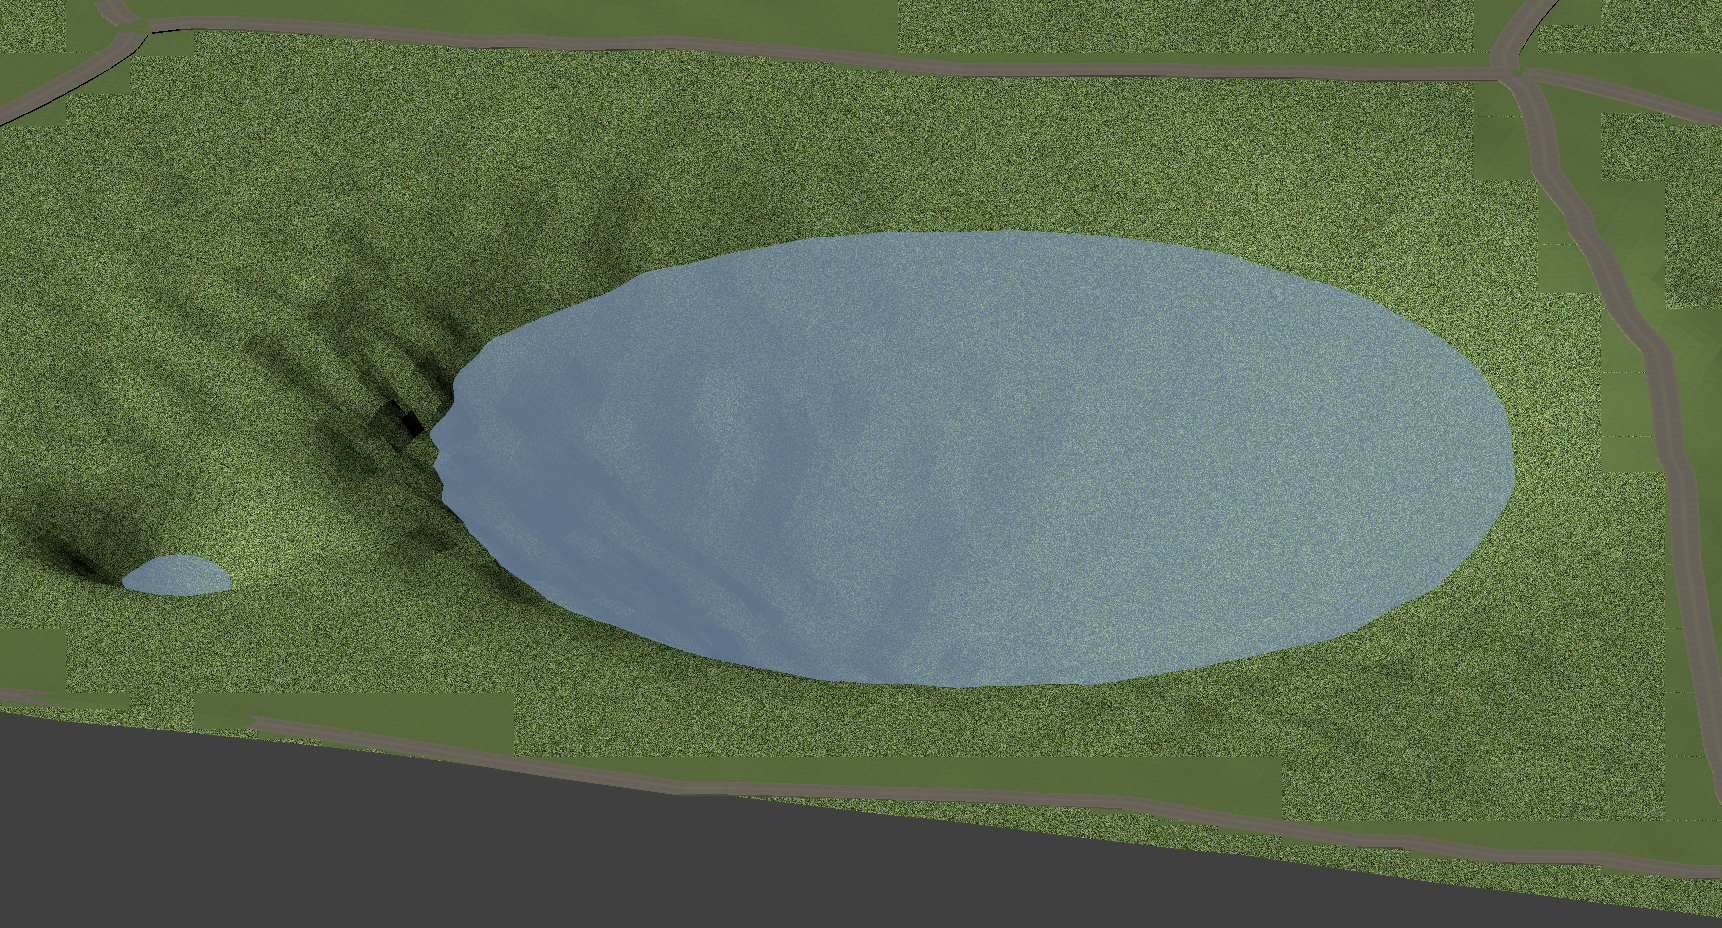
\includegraphics[width=\textwidth]{lake.png}
\caption{Lake city cell}
\label{fig:lake}
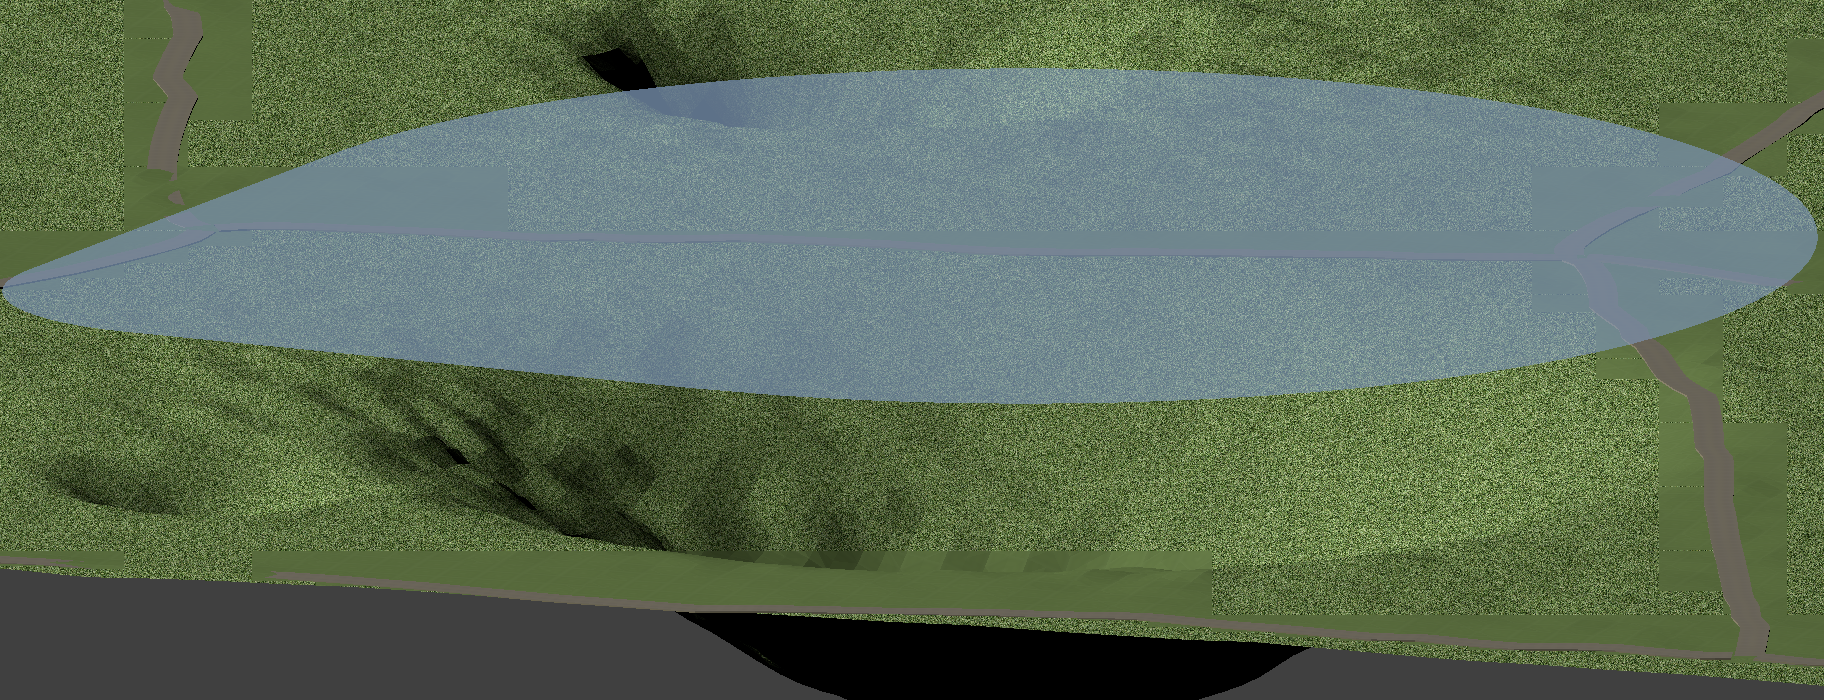
\includegraphics[width=\textwidth]{lake_hull.png}
\caption{Shape of water surface}
\label{fig:lake_hull}
\end{figure}

The planar water surface is mostly hidden under the terrain, and intersects it at the lake shores. It should be kept as small as possible: If it were the entire size of the cell, it could stick out of the terrain, depending on how uneven the terrain is. The convex hull of the lake shores is taken , and expanded by some distance, as shown in figure \ref{fig:lake_hull}.


\subsection{Secondary Roads}
The other 3 kinds of city cells contain secondary roads and buildings. The secondary roads are \emph{grown} inwards into the city cell from several points simulteneously. To start with, the program chooses 2 or more (depending on cell type) \emph{starting points} on the enclosing primary road cycle. From each one of those, a first secondary road segment is added pointing inwards. The two end points of these new segments are called the \emph{extremities}.  

From each extremity point, $n$ new segments are added, pointing at different angles inside a total \emph{span angle}. Their angles are randomly distributed in the span angle by a normal distribution with some deviation. For each of those new proposed segments, a \emph{snap test} is performed to see if the new segment would cross an existing segment, cross a primary street, or come too close (within snap distance) to an existing road. There checks are performed in three steps, as detailed in \cite{Kell2007}. If the result is negative, the new segment is added. If the result is positive, the segment is either discarded, or a segment joining the extremity with the existing road is added instead. The choice is determined by a fixed probability. This procedure is executed for each extremity point alternately, and repeated until there are no more extremity points. The figures \fig{fig:sec1} to \fig{fig:secF} illustrate a stepwise execution of this algorithm.

\begin{figure}[h]
\center
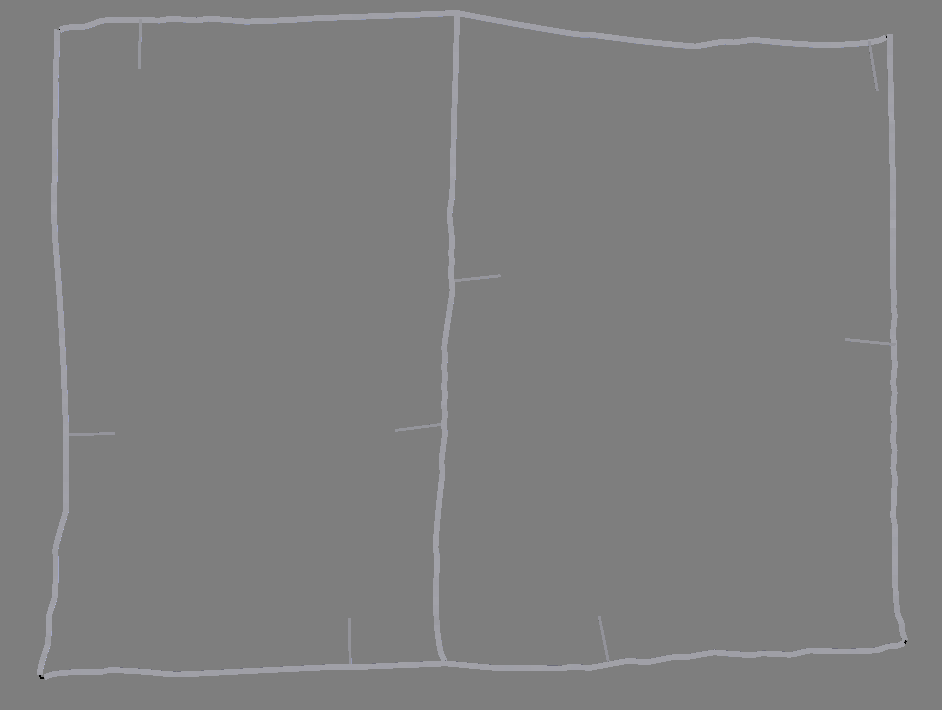
\includegraphics[width=7cm]{s0.png}
\caption{Secondary road growth: Step 0}
\label{fig:sec0}
\end{figure}

\begin{figure}[h]
\center
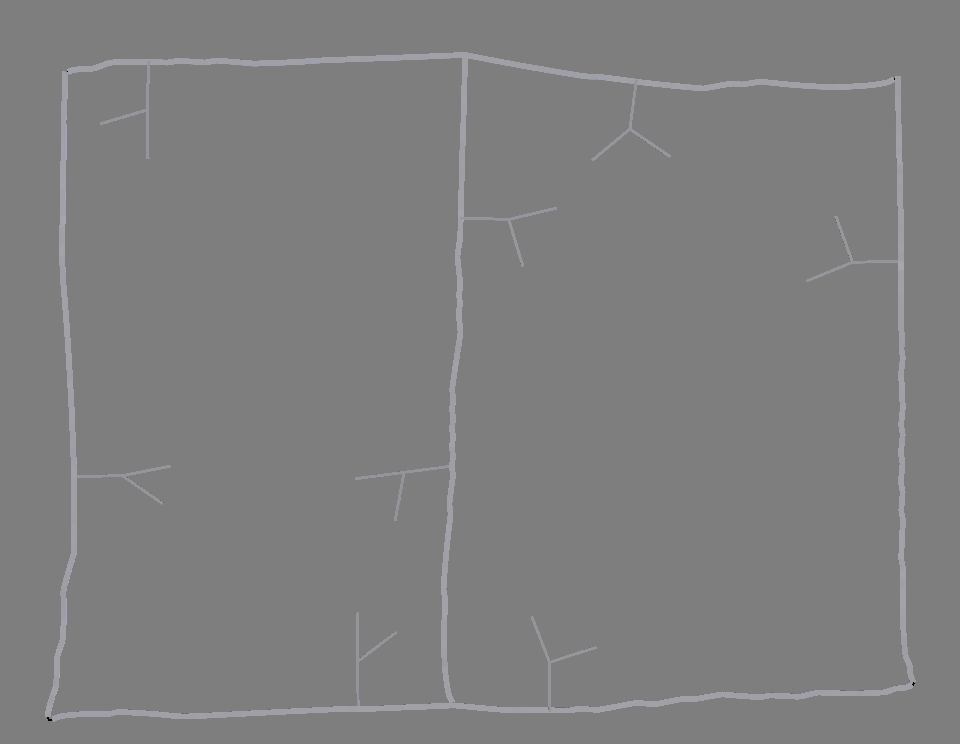
\includegraphics[width=7cm]{s1.png}
\caption{Secondary road growth: Step 1}
\label{fig:sec1}
\end{figure}

\begin{figure}[h]
\center
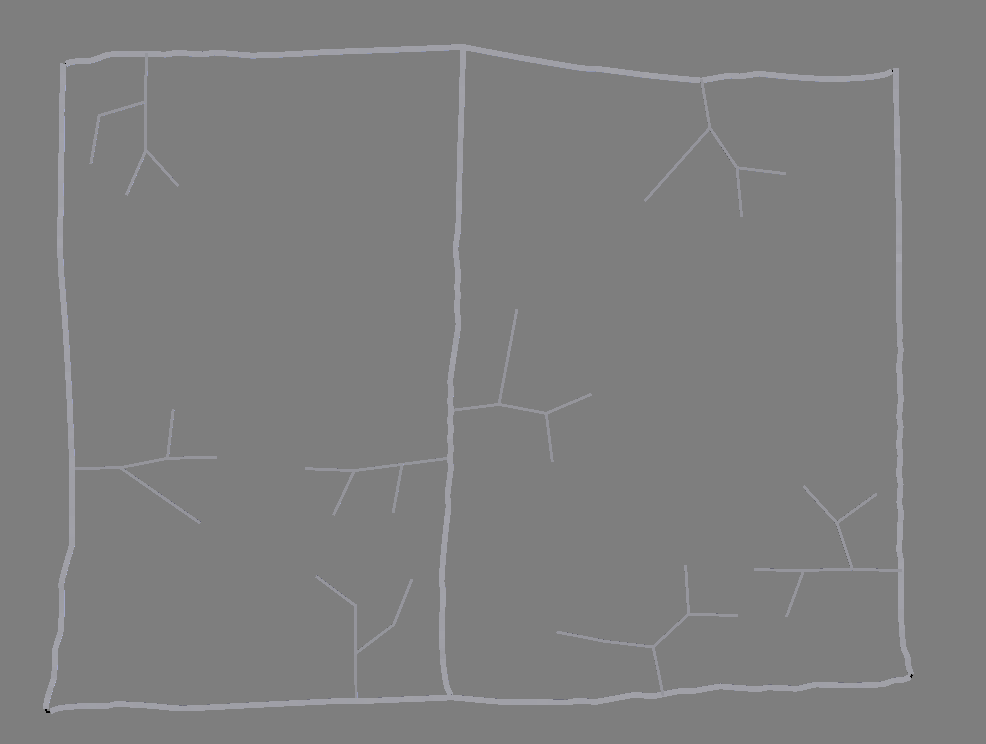
\includegraphics[width=7cm]{s2.png}
\caption{Secondary road growth: Step 2}
\label{fig:sec2}
\end{figure}

\begin{figure}[h]
\center
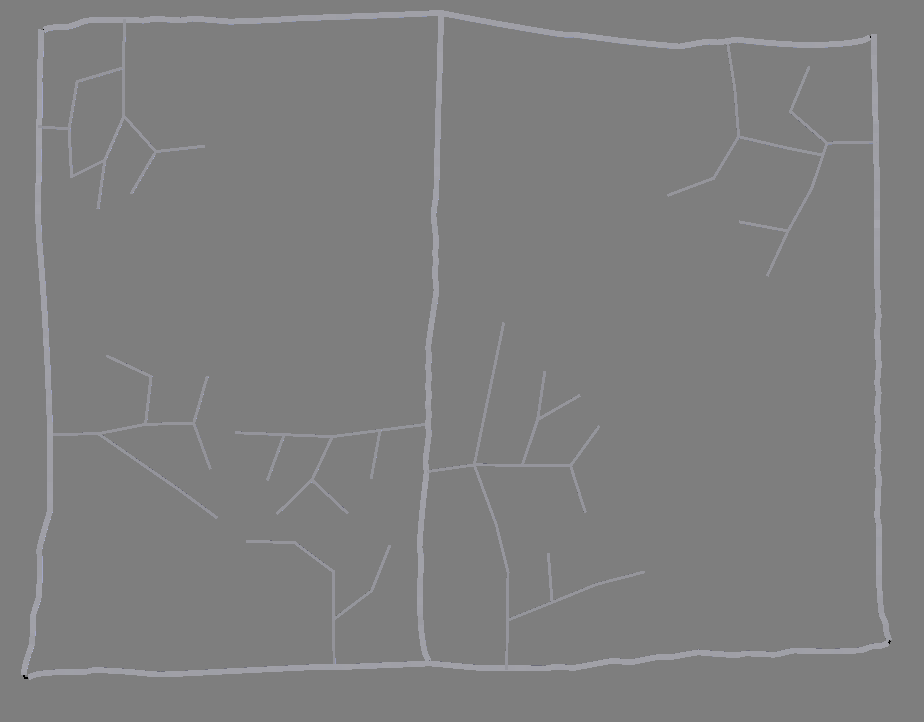
\includegraphics[width=7cm]{s3.png}
\caption{Secondary road growth: Step 3}
\label{fig:sec3}
\end{figure}

\begin{figure}[h]
\center
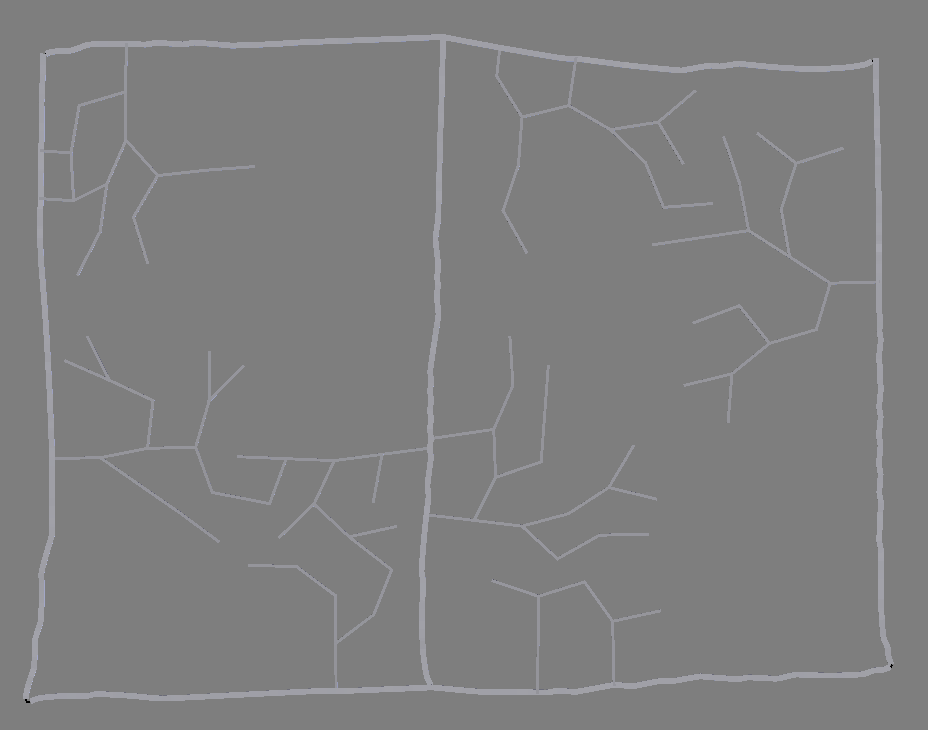
\includegraphics[width=7cm]{s4.png}
\caption{Secondary road growth: Step 4}
\label{fig:sec4}
\end{figure}

\begin{figure}[h]
\center
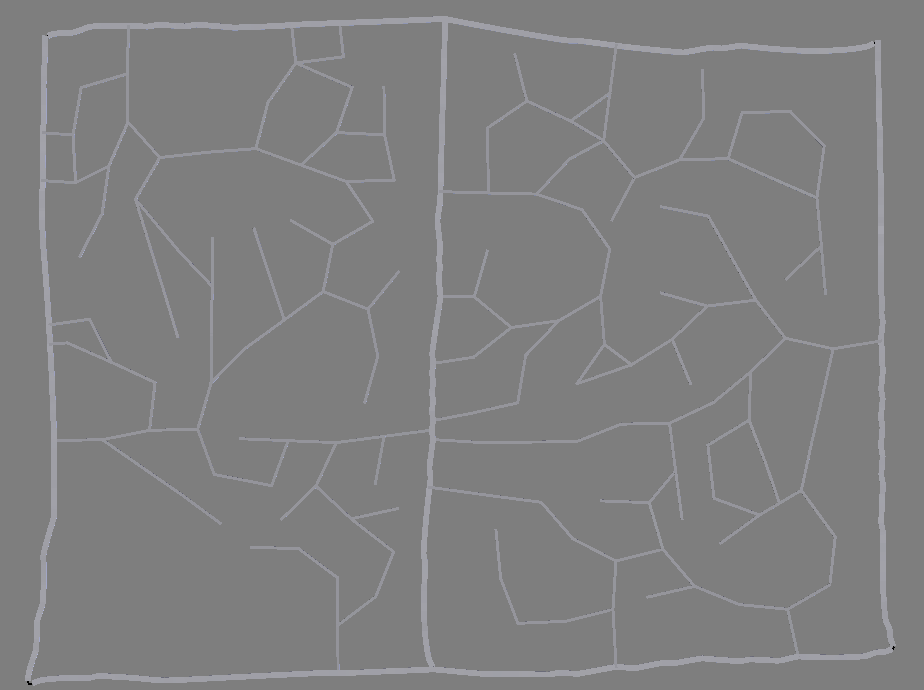
\includegraphics[width=7cm]{sF.png}
\caption{Secondary road growth: End result}
\label{fig:secF}
\end{figure}

The parameters for the algorithm are chosen depending on the type of cell:

\begin{tabular}{l | c | c | c}
	\textbf{Cell type} & \textbf{Urban} & \textbf{Suburban} & \textbf{Rural} \\
	\hline 
	Starting points & 2 & 4 & 7 \\
	Segment size & 30 m & 30 m & 50 m \\
	Snap size & 20 m & 20 m & 30 m \\
	Number of new segments & 3 & 2 & 2 \\
	Span Angle & 270 deg & 216 deg & 144 deg \\
	Angle deviation & 0 & 0.5 & 0.5 \\
	Join Probability & 100\% & 40\% & 20\% \\
\end{tabular}

The parameters for urban cells produce a checkerboard pattern: Angles of -90, 0 and +90 degrees are forced, and the new segments are always joined to existing ones where possible. The different outcomes for the three cell types are shown in figures \fig{fig:cellU}, \fig{fig:cellS} and \fig{fig:cellR}.

\begin{figure}[h]
\center
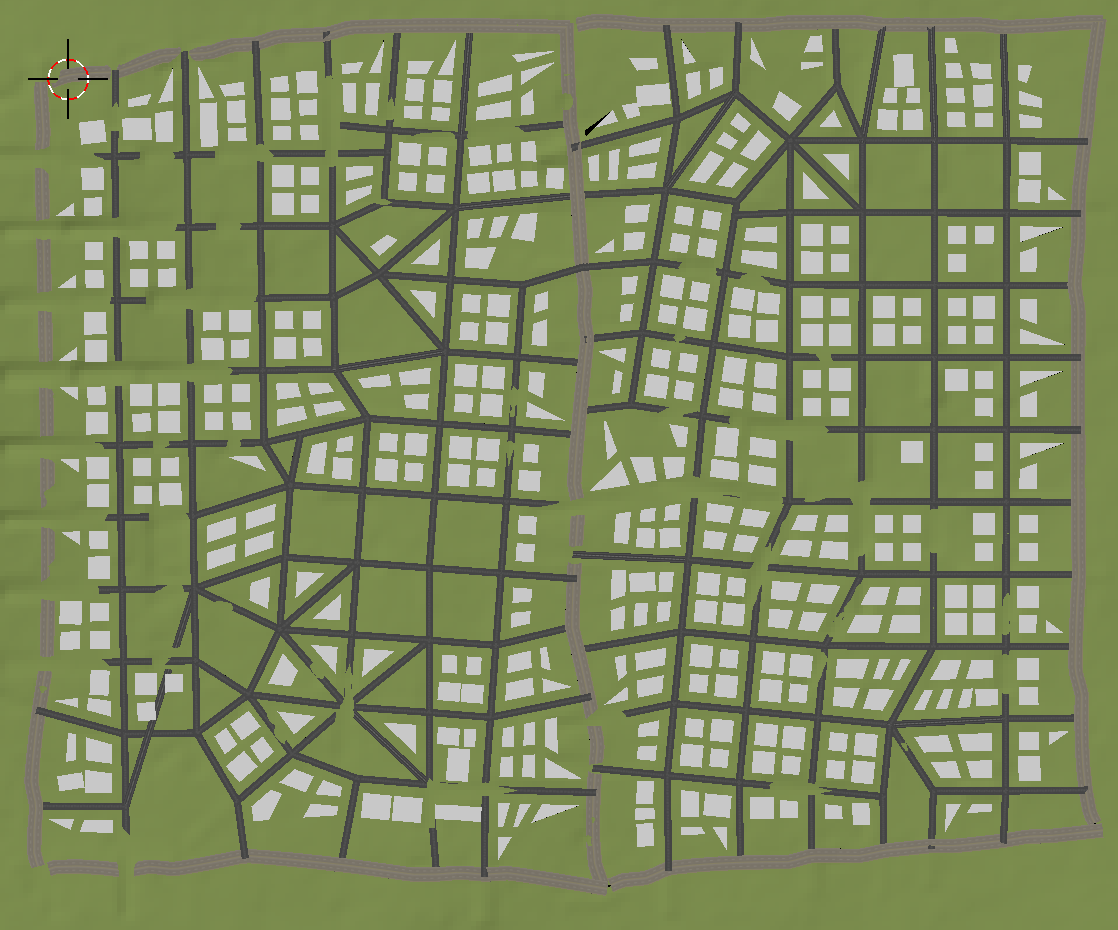
\includegraphics[width=\textwidth]{cellU.png}
\caption{Urban city cell}
\label{fig:cellU}
\end{figure}

\begin{figure}[h]
\center
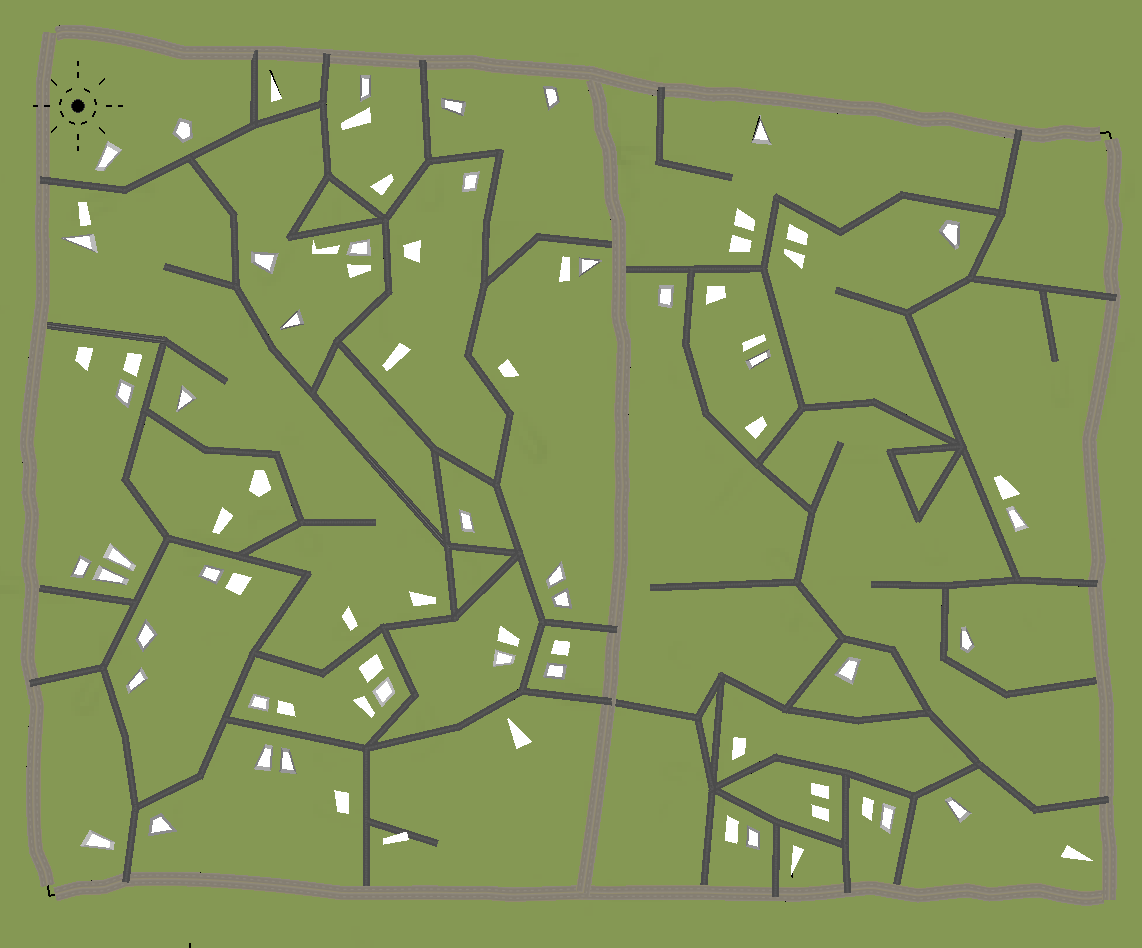
\includegraphics[width=\textwidth]{cellS.png}
\caption{Suburban city cell}
\label{fig:cellS}
\end{figure}

\begin{figure}[h]
\center
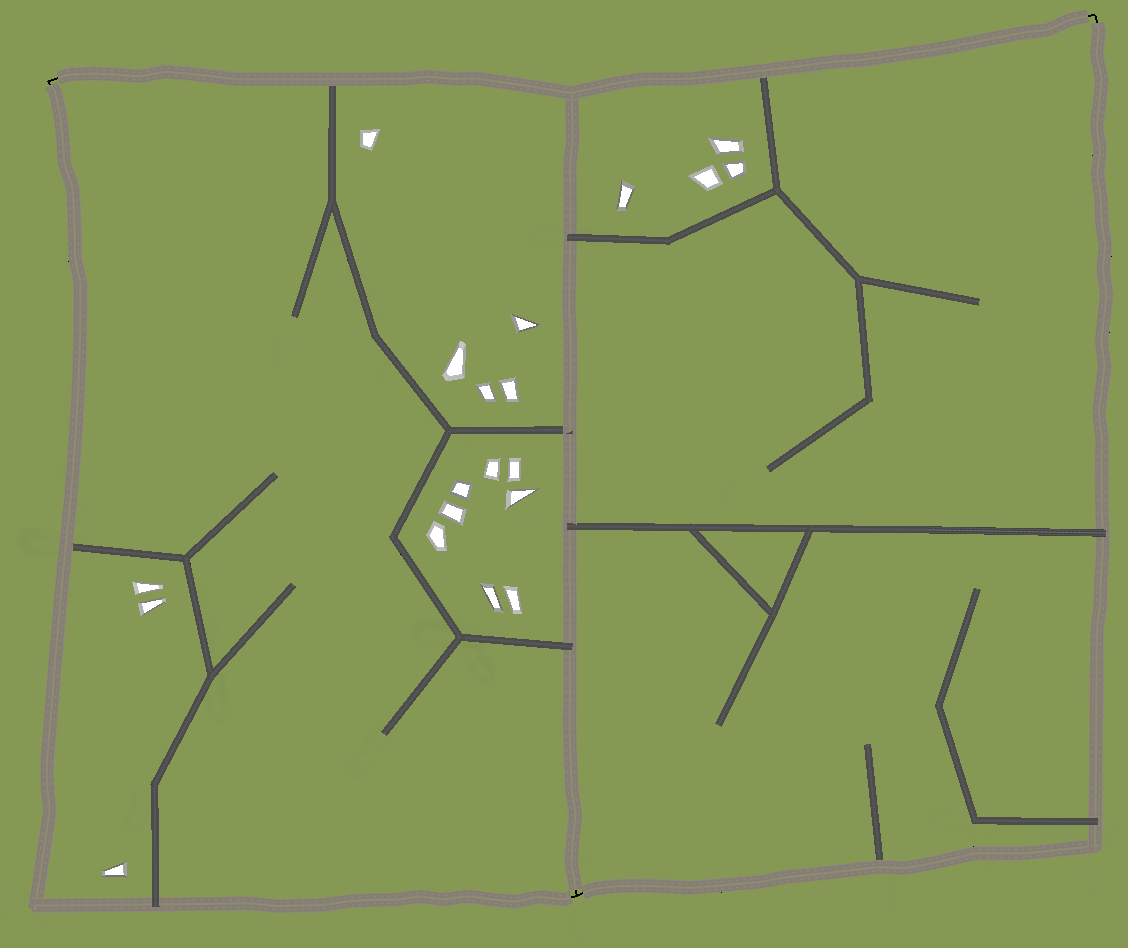
\includegraphics[width=\textwidth]{cellR.png}
\caption{Rural city cell}
\label{fig:cellR}
\end{figure}

In order to avoid roads going under a noisy terrain, the terrain is flattened and embossed around both the secondary and primary roads.


\subsection{Blocks}
The regions enclosed by the secondary roads are called \emph{blocks}. Buildings will be placed inside blocks. To find the blocks, the first step is to generate a graph consisting of the secondary roads of the cell, and the primary street cycle of the surrounding primary streets. The X, Y coordinates give an embedding of this planar graph. Finding the enclosed regions corresponds to finding the \emph{minimal cycle basis} on this graph embedding. For this the algorithm described in \cite{Eber2005} is implemented. A minimal cycle basis (MCB) is the unique set of cycles in a graph such that all other cycles can be constructed by an exclusive-OR operation on a subset of the MCB.

After the MCB has been calculated, get the polygon corresponding to each cycle. In order to simulate a sidewalk, the polygon is contracted by some decimeters. For this each edge of the polygon is moved inwards, parallel to the original, by that distance. Then a new polygon is constructed from the intersection points of these new lines. An equivalent method is used for expanding polygons at some positions in the program. The size of the sidewalk also depends on the cell type.

The next step is to subdivide the blocks into \emph{lots}. This is done by subdividing the blocks by two using a recursive algorithm: The longest side of the block, and the side most parallel to it are taken. The block is cut in two through the midpoints of those two edges. The process is repeated recursively on the two halves, until the area of the remaining region is less than a given minimum, of it has less than 4 sides. Figure \ref{fig:alllots} shows the result of this procedure.

\begin{figure}[h]
\center
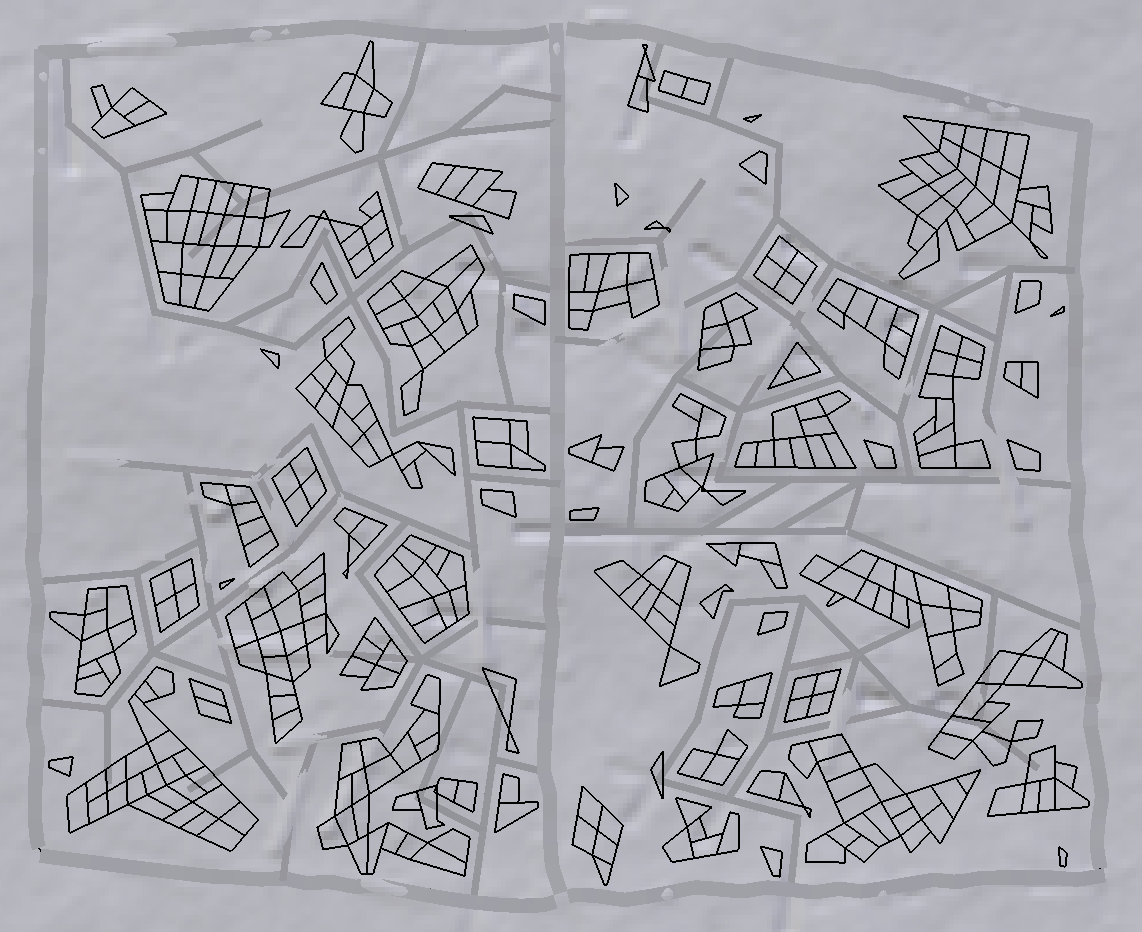
\includegraphics[width=\textwidth]{alllots.png}
\caption{Dividing blocks into lots, without filtering. Contains errors due to bug in program.}
\label{fig:alllots}
\end{figure}

The lots will each contain a building. Because buildings should only be placed news to roads, an additional filter is applied: At each iteration, the sides that are adjacent to a road are remembered, and blocks/lots during the recursion that are no longer adjacent to a road are discarded. \ref{fig:lots} shows the remainer after this filtering.

\begin{figure}[h]
\center
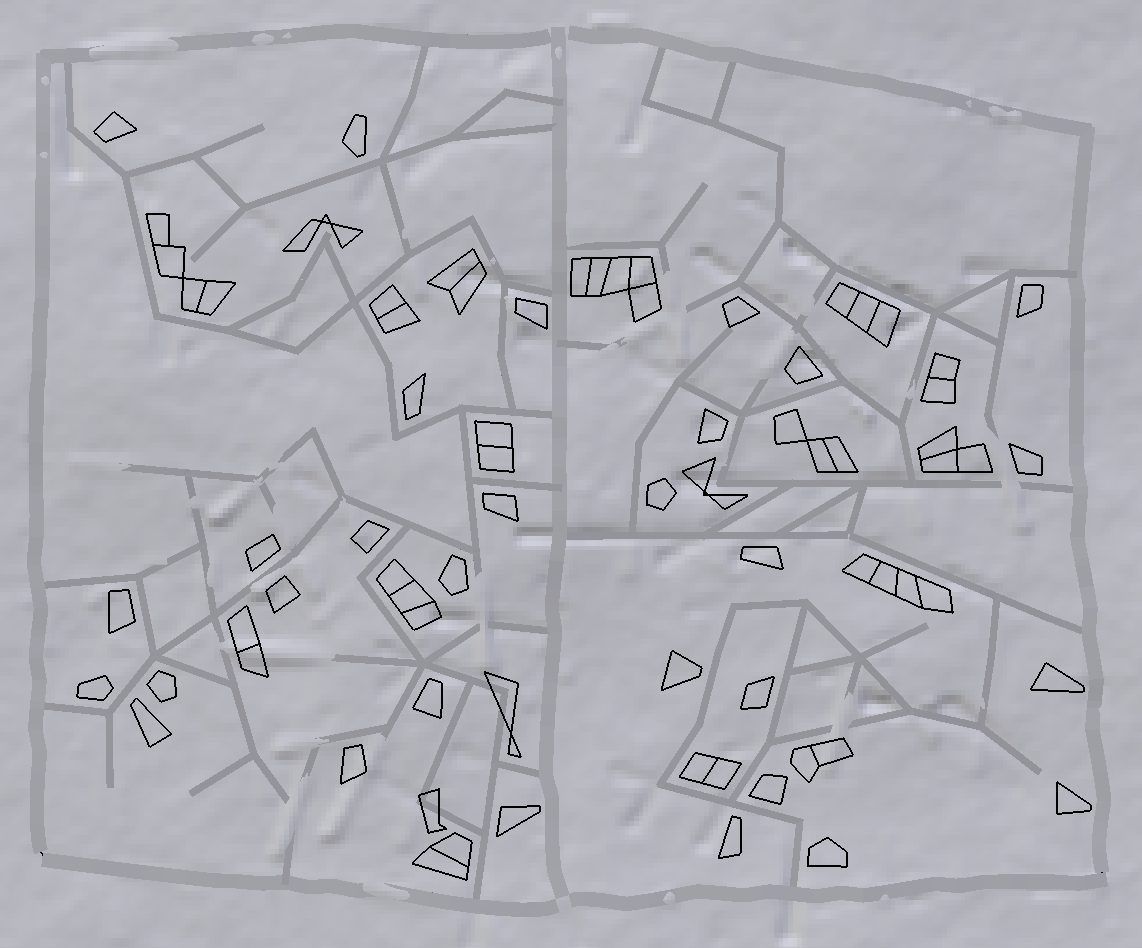
\includegraphics[width=\textwidth]{lots.png}
\caption{Dividing blocks into lots, with filtering.}
\label{fig:lots}
\end{figure}


\subsection{Buildings}
Three kinds of buildings are implemented: Skyscrapers, Offices and Houses. Each building is placed on a lot.

Both offices and houses consist simply of an extrusion of the lot shape, after it has been contracted by some decimeters. For houses, a slanted roof is added on top. Offices are taller and have a flat roof.

Skyscrapers are generated using a recursive algorithm similar to what's described in \cite{Pari2001}. In the article a method is presented to describe complex building shaping mechanisms using an \emph{L-System} operating on a grammar. The algorithm here simple operated recursively on in two steps:

Starting with a bounding box, the upper rectangle is cut with another, slightly smaller rectangle. The remaining part is sliced/intruded downwards down to a given base height. Then the procedure is repeated with the remaining tower bounding box. During the first half of the process, the base is chosen at the lower range, during the second half, it is at the upper range. The results can be seen in the screenshots.


\section{Implementation}
\label{sec:implementation}
The program consists of a Blender add-on. Some details regarding the implementation of the algorithms in Blender:
\begin{itemize}
\item The code is modular and object-oriented. The city is represented as a composition of objects representing the whole city, a city cell, a block and a building.
\item The generation of the city happens in two stages. First an internal representation is generated, using \texttt{City.generate()}. During this process the random number generator is used and the composition of objects holding the city is created. No Blender objects are created or used. As a result, it would be easily possible to uncouple the program from Blender.
\item After the internal representation has been generated, the recursive call to \\ \texttt{City.create\_blender\_object()} generates a hierarchy of Blender objects for the city. This process no longer uses the random number generator and thus it is entirely deterministic.
\item All randomization is based on the Python \texttt{random} random number generator. Thus by setting the same seed value, the exact same city will be generated. The functionality to explicitly define a seed is included in the user interface.
\item All of the \texttt{create\_blender\_object} process operates on Blender \textt{data}, and never on \texttt{operators}.
\item For the primary streets, a premade, textured segment from \texttt{assets.blender} is imported into the scene. Then it is chained to itself $n$ times using the \emph{Array} modifier, and the chain is aligned to a road using the \emph{Curve} modifier.
\item For secondary roads which remain straight, the premade segment is scaled in one direction, and then aligned to the line segment using the \emph{Curve} modifier. The scale of the texture needs to be readjusted to remain constant with regard to the scene.
\item The roads segments with their meshes and their textures are \emph{linked} from the \texttt{assets.blender} file. As a result no unnecessary copies of it are made in-memory.
\tem The \emph{NetworkX} (\url{https://networkx.github.io}) Python library is used and needs to be installed into Blender's python distribution.
\end{itemize}

\subsection{Problems}
Due to time constraints and other problems, the project is unfinished and there are several bugs and errors in the implementations. The main remaining problems:
\begin{itemize}
\item The buildings are untextured. However, texturization would be relatively simple to add, since adding a texture and possibly a bump map to the facades of the buildings could already give a realistic effect on the large scale.
\item There are bugs in the program. In rare cases it loops infinitly or crashes.
\item There are some problems remaining with the \emph{minimal cycle basis} implementation in \texttt{mcb.py}. Because of the combinatorial complexity, this algorithm is hard to debug by simple testing.
\item The algorithm used to expand and contract polygons is not correct in all cases and leads to the results seen in figure \ref{fig:alllots}. Sometimes buildings can have incorrect shapes (non-simple polygons), and cross over roads.
\item Streets are not well adapted to the terrain. They get simply placed near the terrain surface, without taking into consideration the mesh of the terrain. A better implemenentation could ``draw'' the streets onto the terrain surface, and then extrude from it.
\item Likewise, street intersections are not handled well. Different primary/secondary street segments simply intersect each other. However, the chaining of primary road segments is handled correctly because of the \emph{Array} modifier.
\item There is an attempted solution to the terrain-street intersections: The terrain is flattened and embossed slightly below streets. However this still produces incorrect results.
\end{itemize}

\subsection{Installation}
The \emph{NetworkX} (\url{https://networkx.github.io}) Python library is used and needs to be installed into Blender's python distribution. One procedure for this is to install the same version of Python on the host computer as the one that is included with Blender, and the install \emph{NetworkX} using \texttt{pip3.4 install networkx}. After this copy \emph{networkx} from the host's {site-available} directory into Blender's own.

After this the add-on can be installed in Blender, an shows up as in \ref{fig:addon}.

\begin{figure}[h]
\center
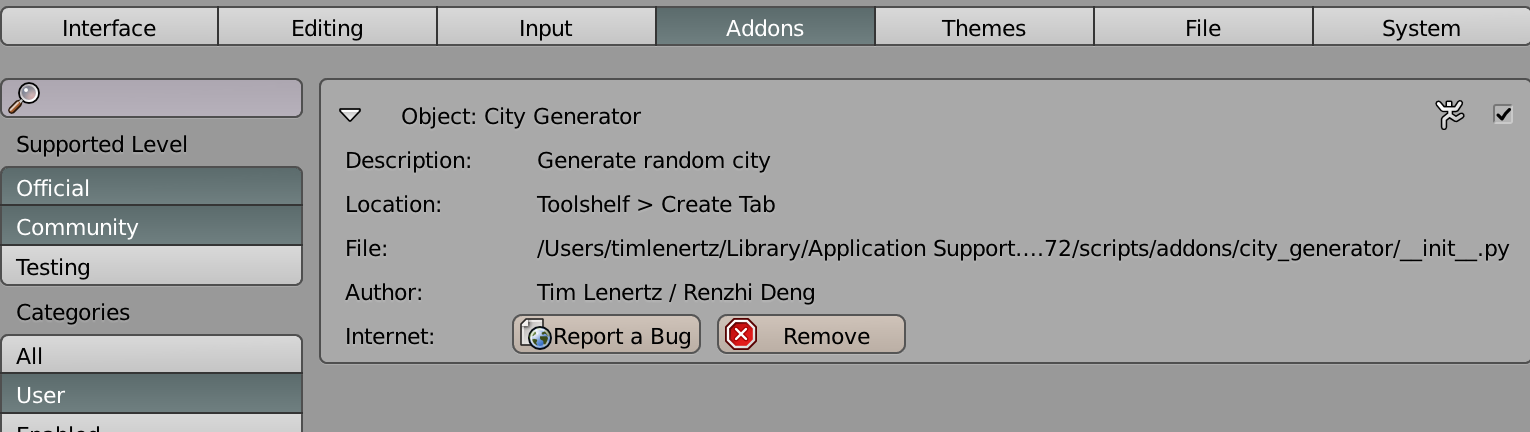
\includegraphics[width=\textwidth]{addon.png}
\caption{The Blender add-on.}
\label{fig:addon}
\end{figure}


\section{Usage}
When installed, the panel shown in \ref{fig:param} is displayed in the Blender tool shelf. The following parameters are available:
\begin{description}
\item[Name] Name of the root object of the city to generate. Clicking ``Delete City'' will recursively remove the object of that name and its children.
\item[Random Seed] If non-empty, seed to use for the random number generator. The same seed generate exactly the same city. If empty, it is randomly chosen.
\item[Corner Elevation] Maximal elevation of the four terrain corners. If 0 (default) the terrains remains globally flat, but can have local noise.
\item[Size] Side length of the (square) city terrain in meters.
\item[Elevation] Multiplier for the terrain elevation. Larger value results in more noisy terrain. Zero results in perfectly flat terrain.
\item[Junctions] Approximate number of primary street junctions. Rounded up to allow for $n \cross m$ grid. Determines number of city cells.
\item[Grid Alignment] The higher this setting, the more closely the cells are aligned on a regular grid. See figures \emph{fig:primaryS} and \emph{fig:primaryL}.
\item[Urbanization] The higher this value, the more urban cells generated compared to rural cells.
\end{description}

\begin{figure}[h]
\center
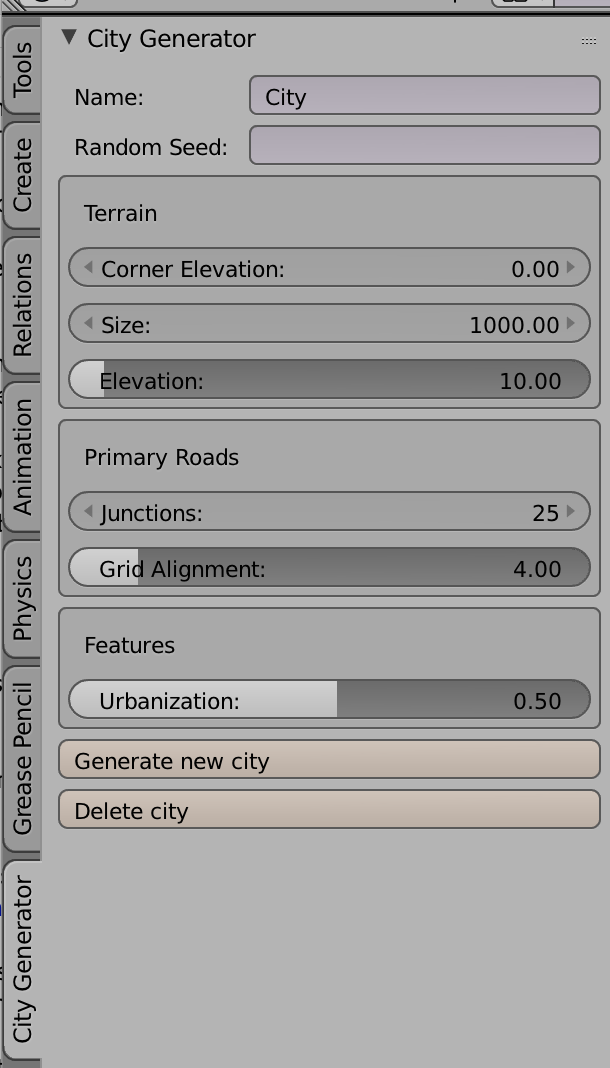
\includegraphics[width=8cm]{param.png}
\caption{Tool shelf panel of the add on.}
\label{fig:param}
\end{figure}

\section{Results}
Some results obtained with the add-on: \\ \\

\center
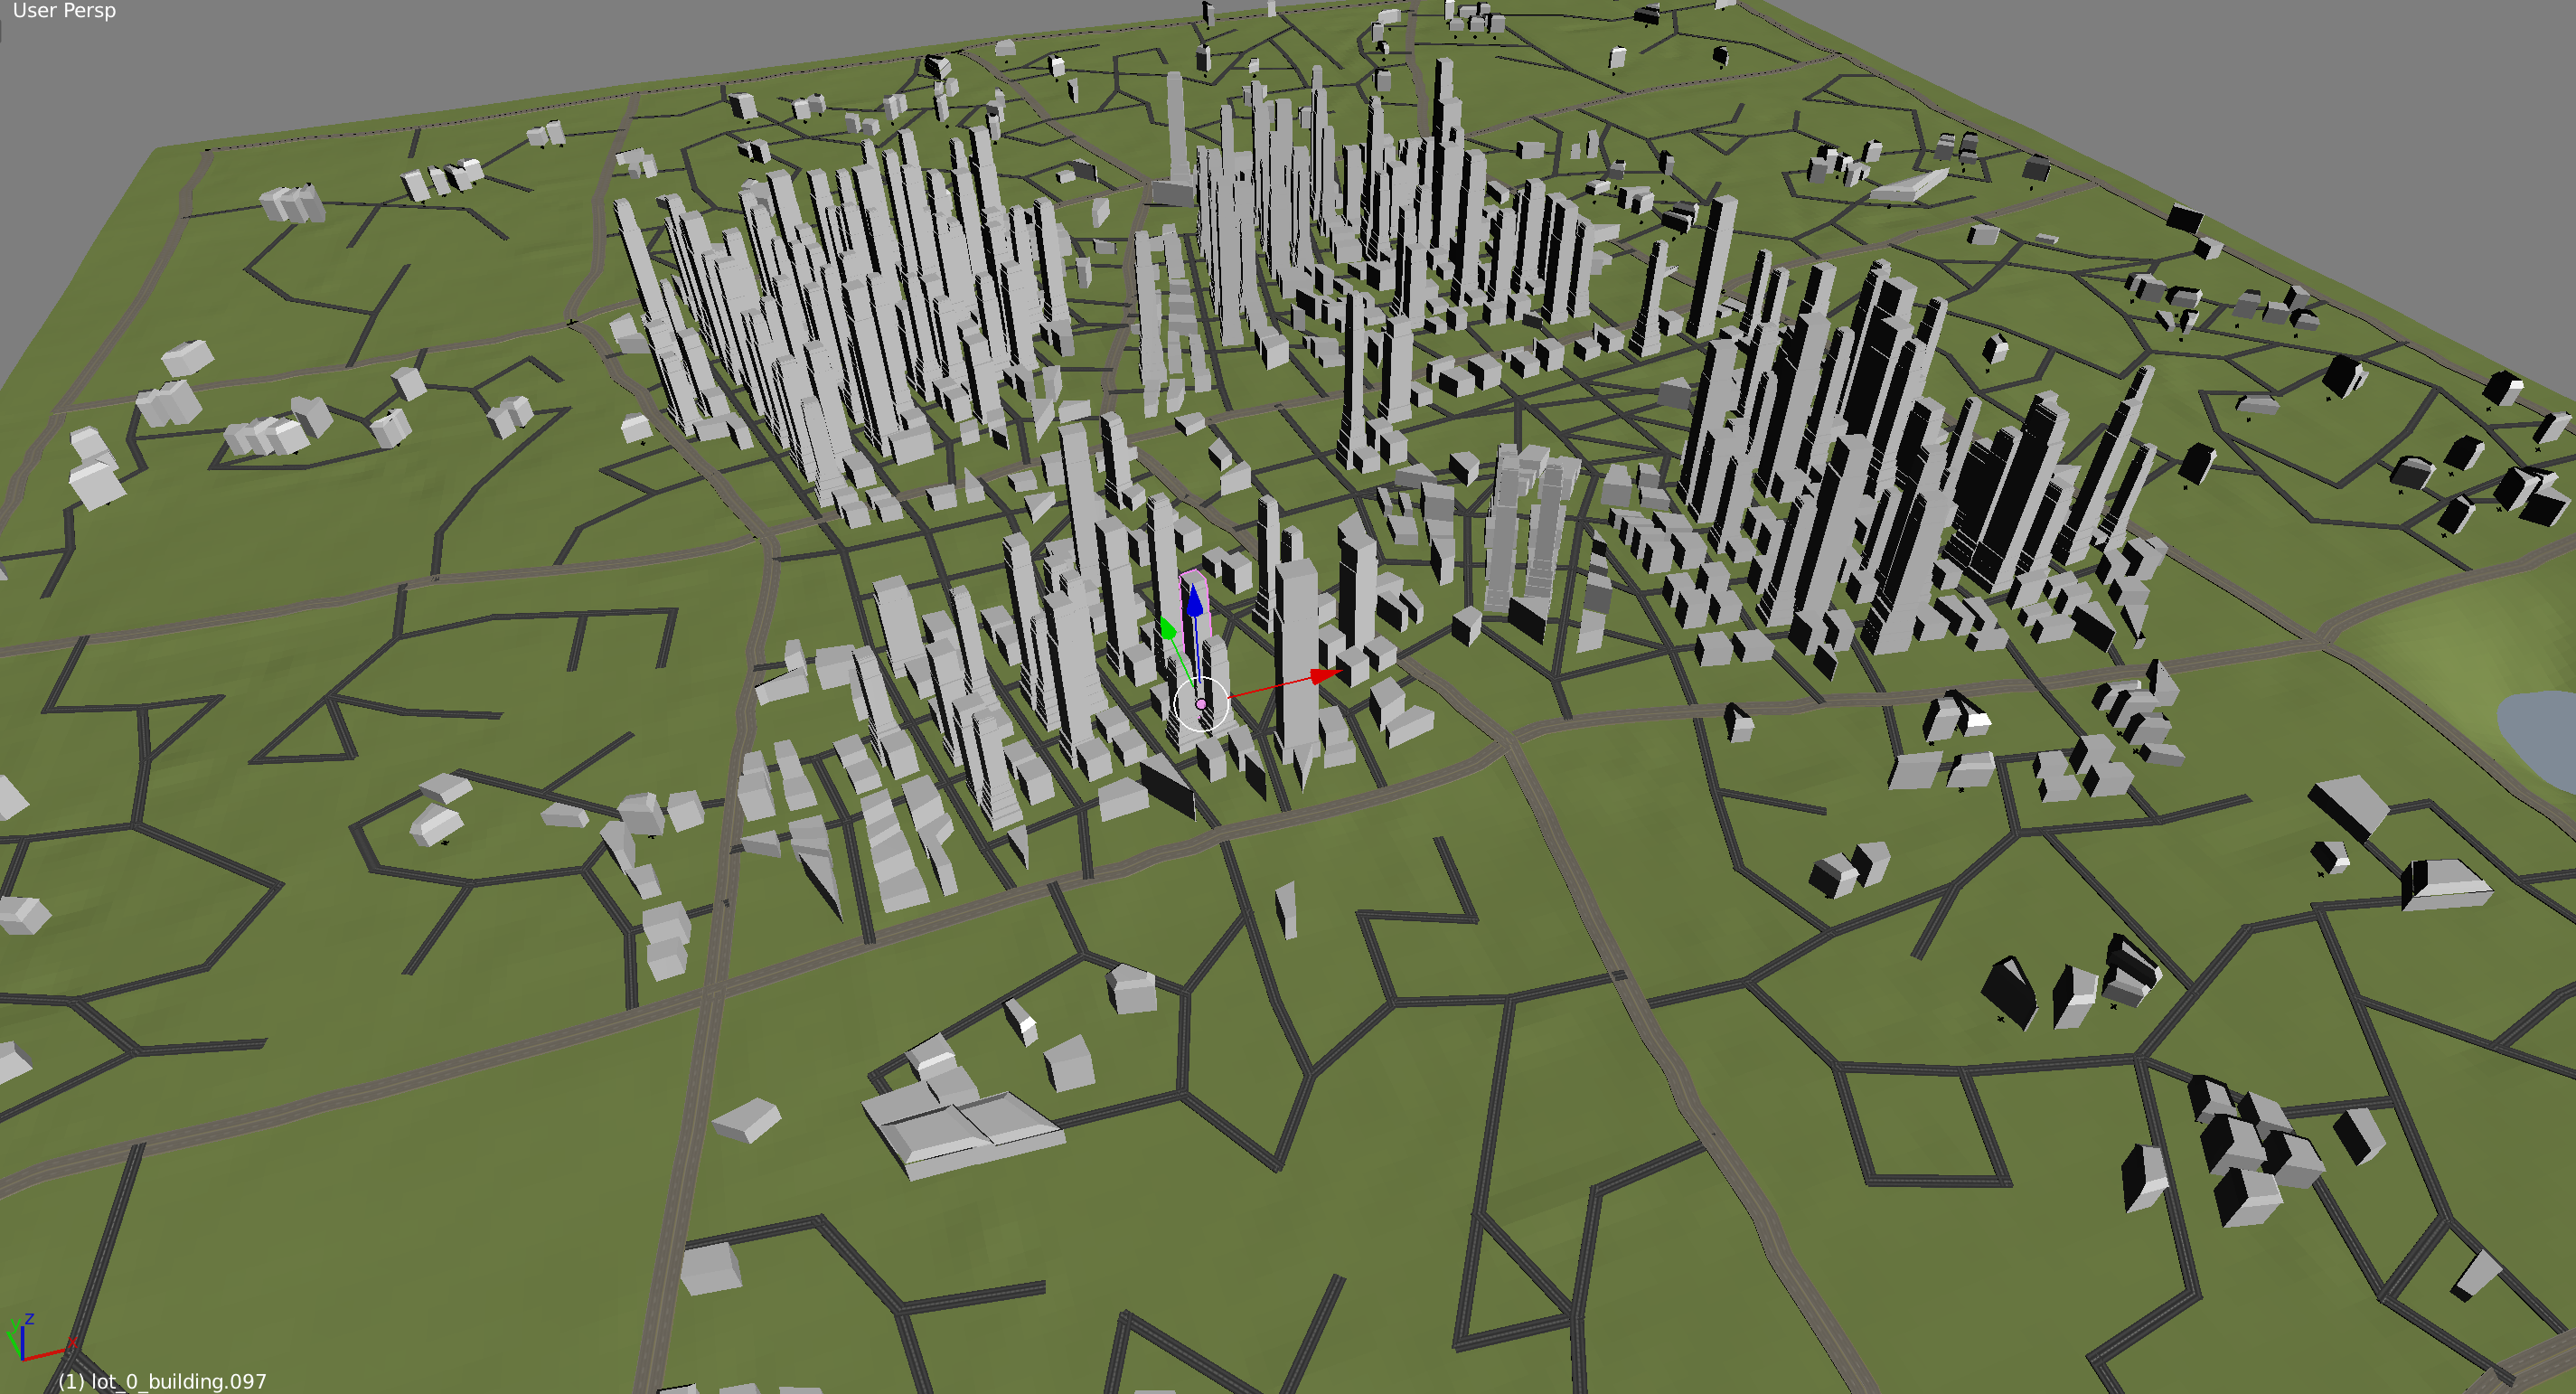
\includegraphics[width=\textheight,angle=90]{view1.png}

\center
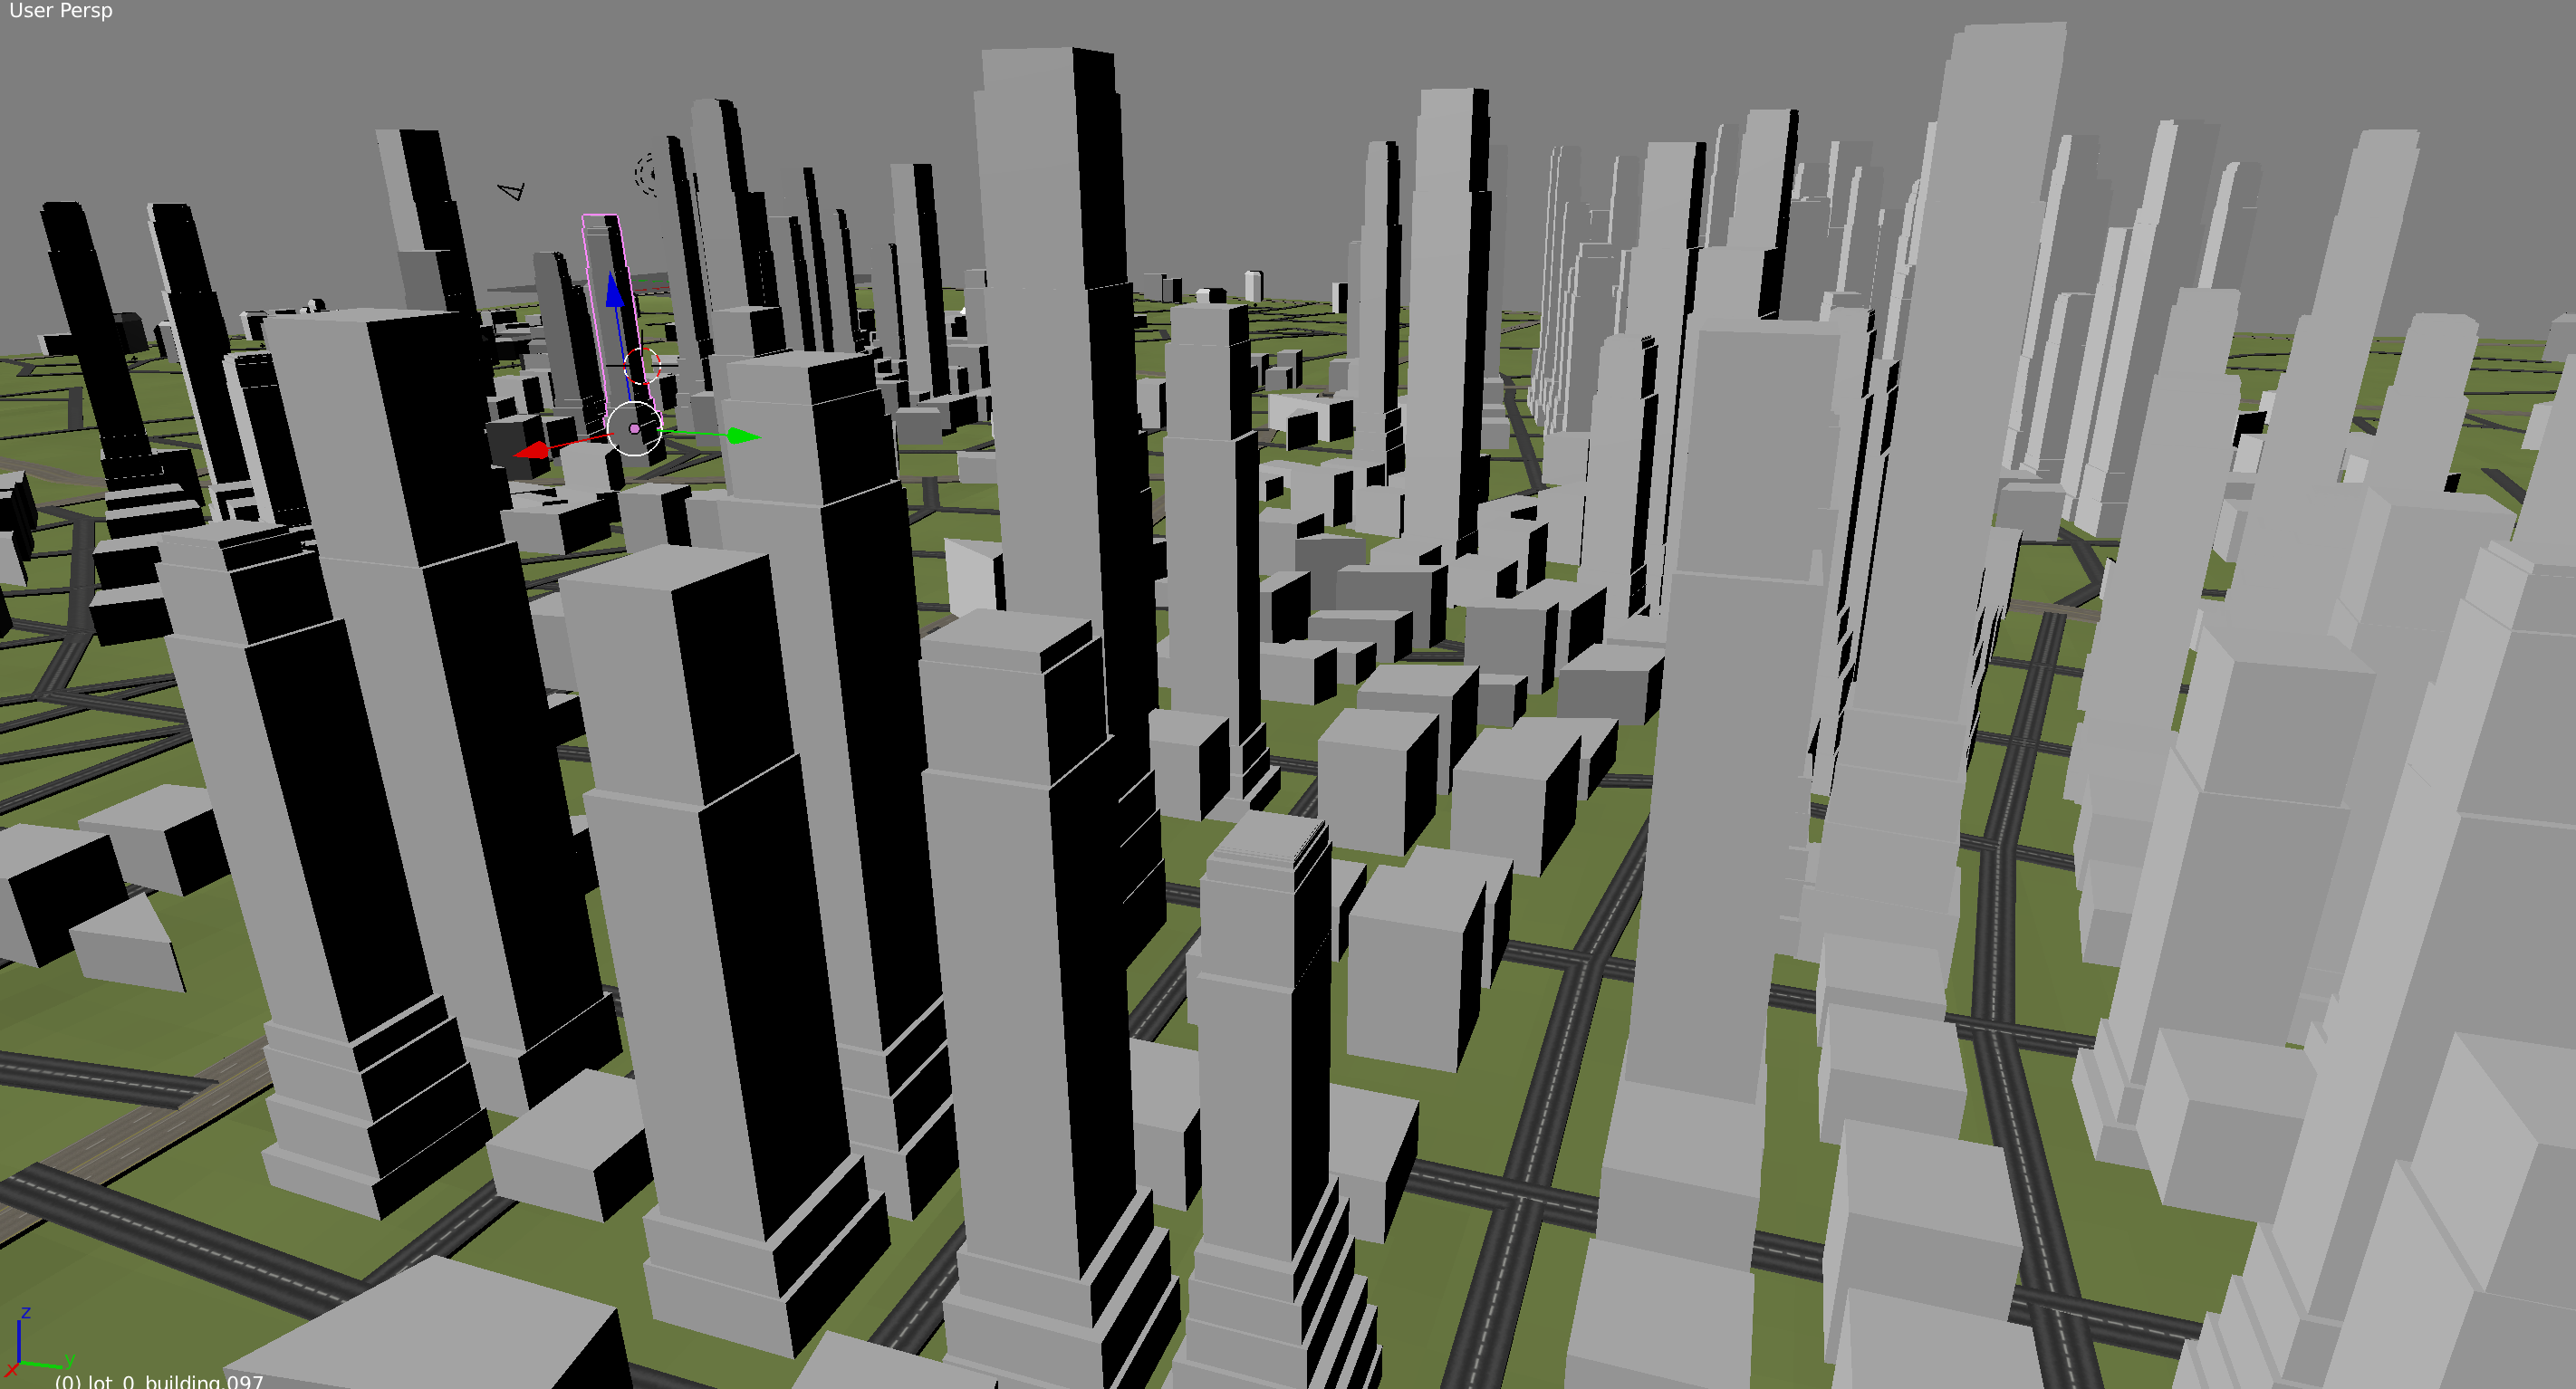
\includegraphics[width=\textheight,angle=90]{view2.png}

\center
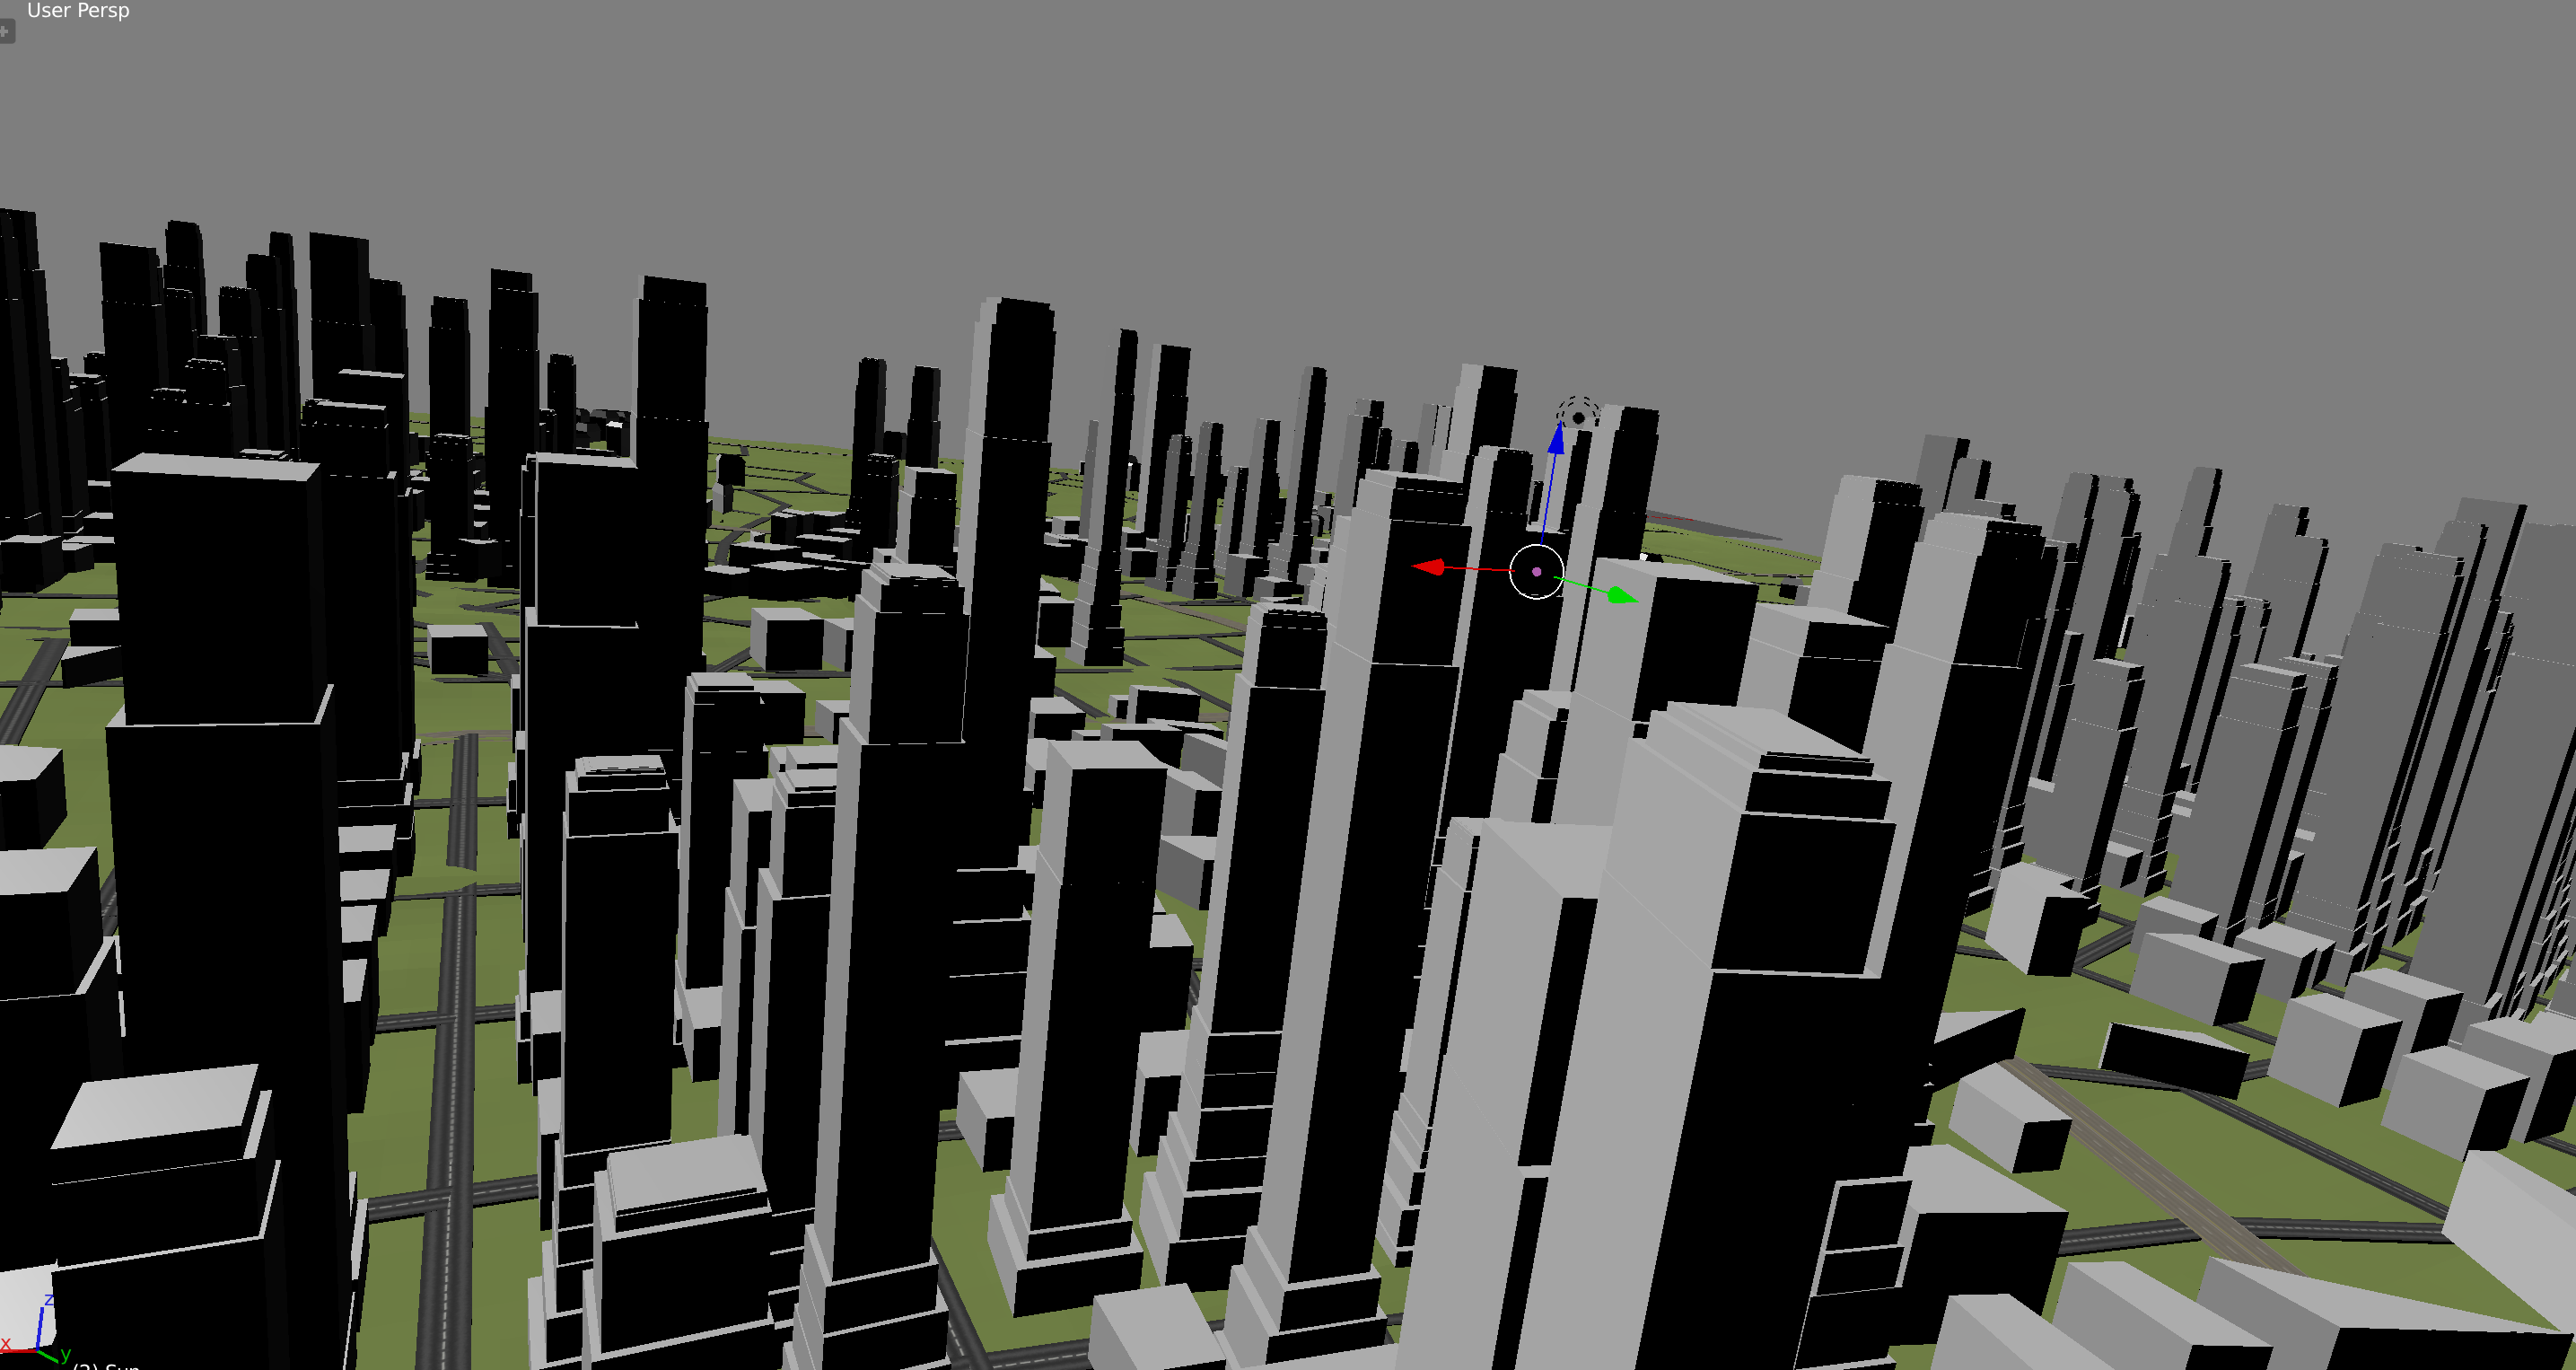
\includegraphics[width=\textheight,angle=90]{view4.png}

\center
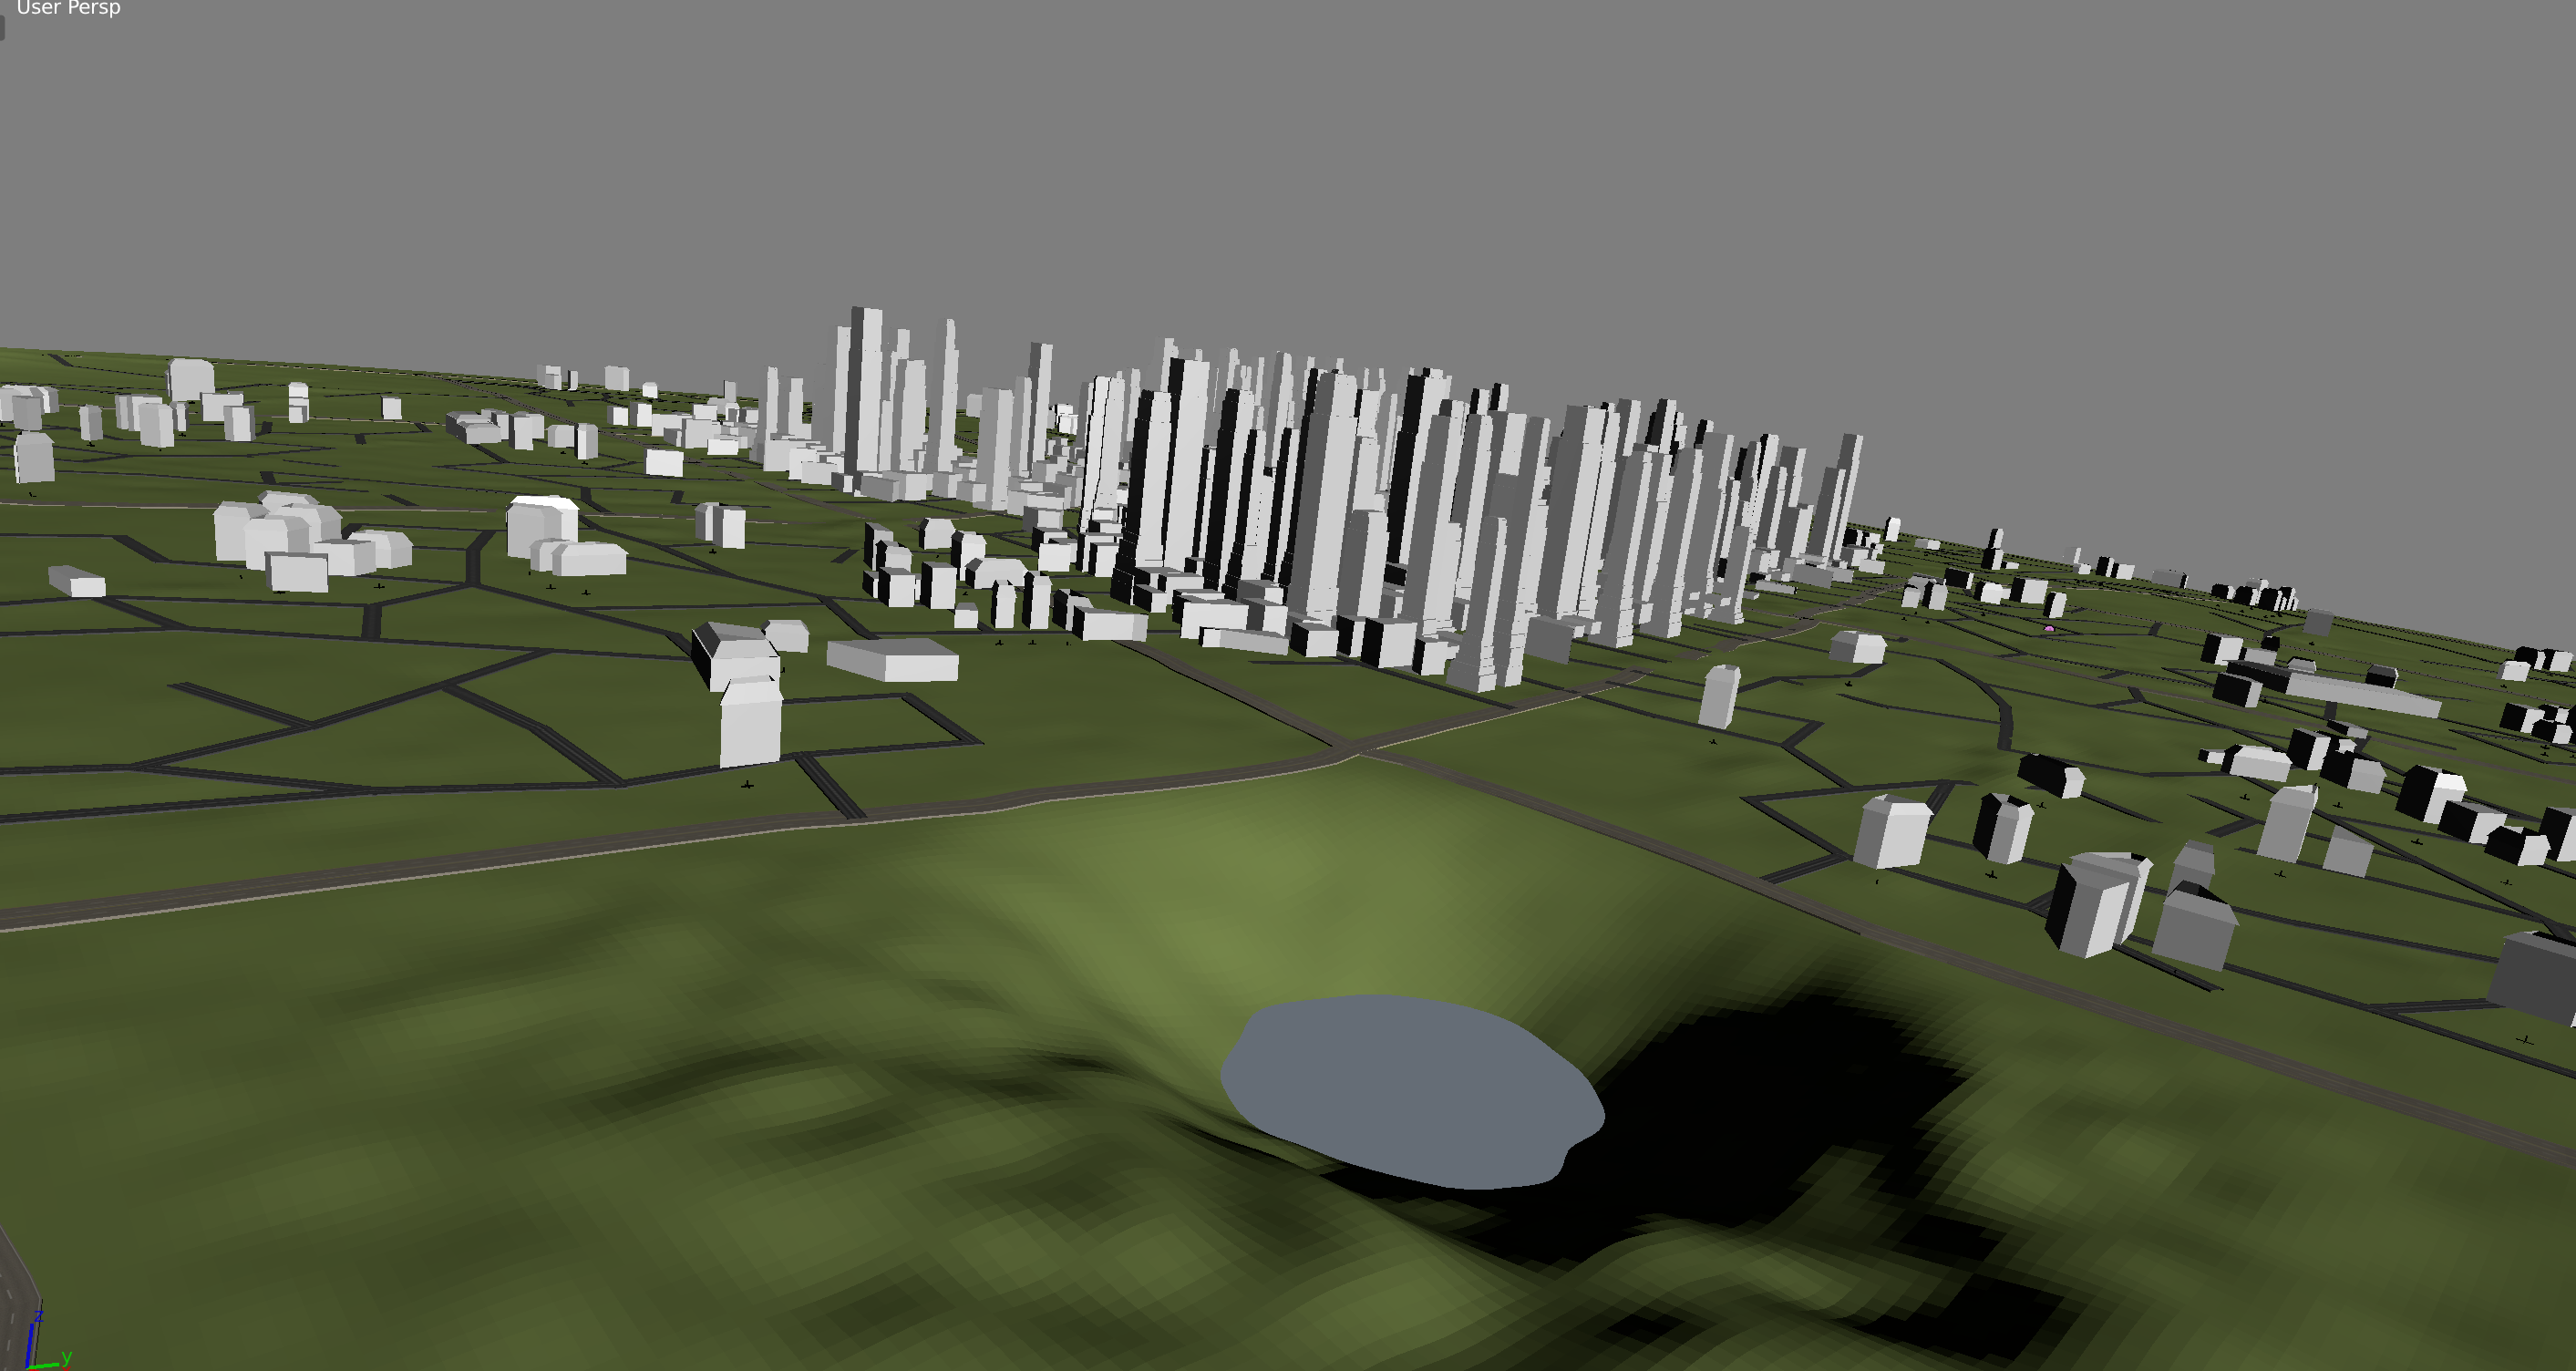
\includegraphics[width=\textheight,angle=90]{view5.png}

\center
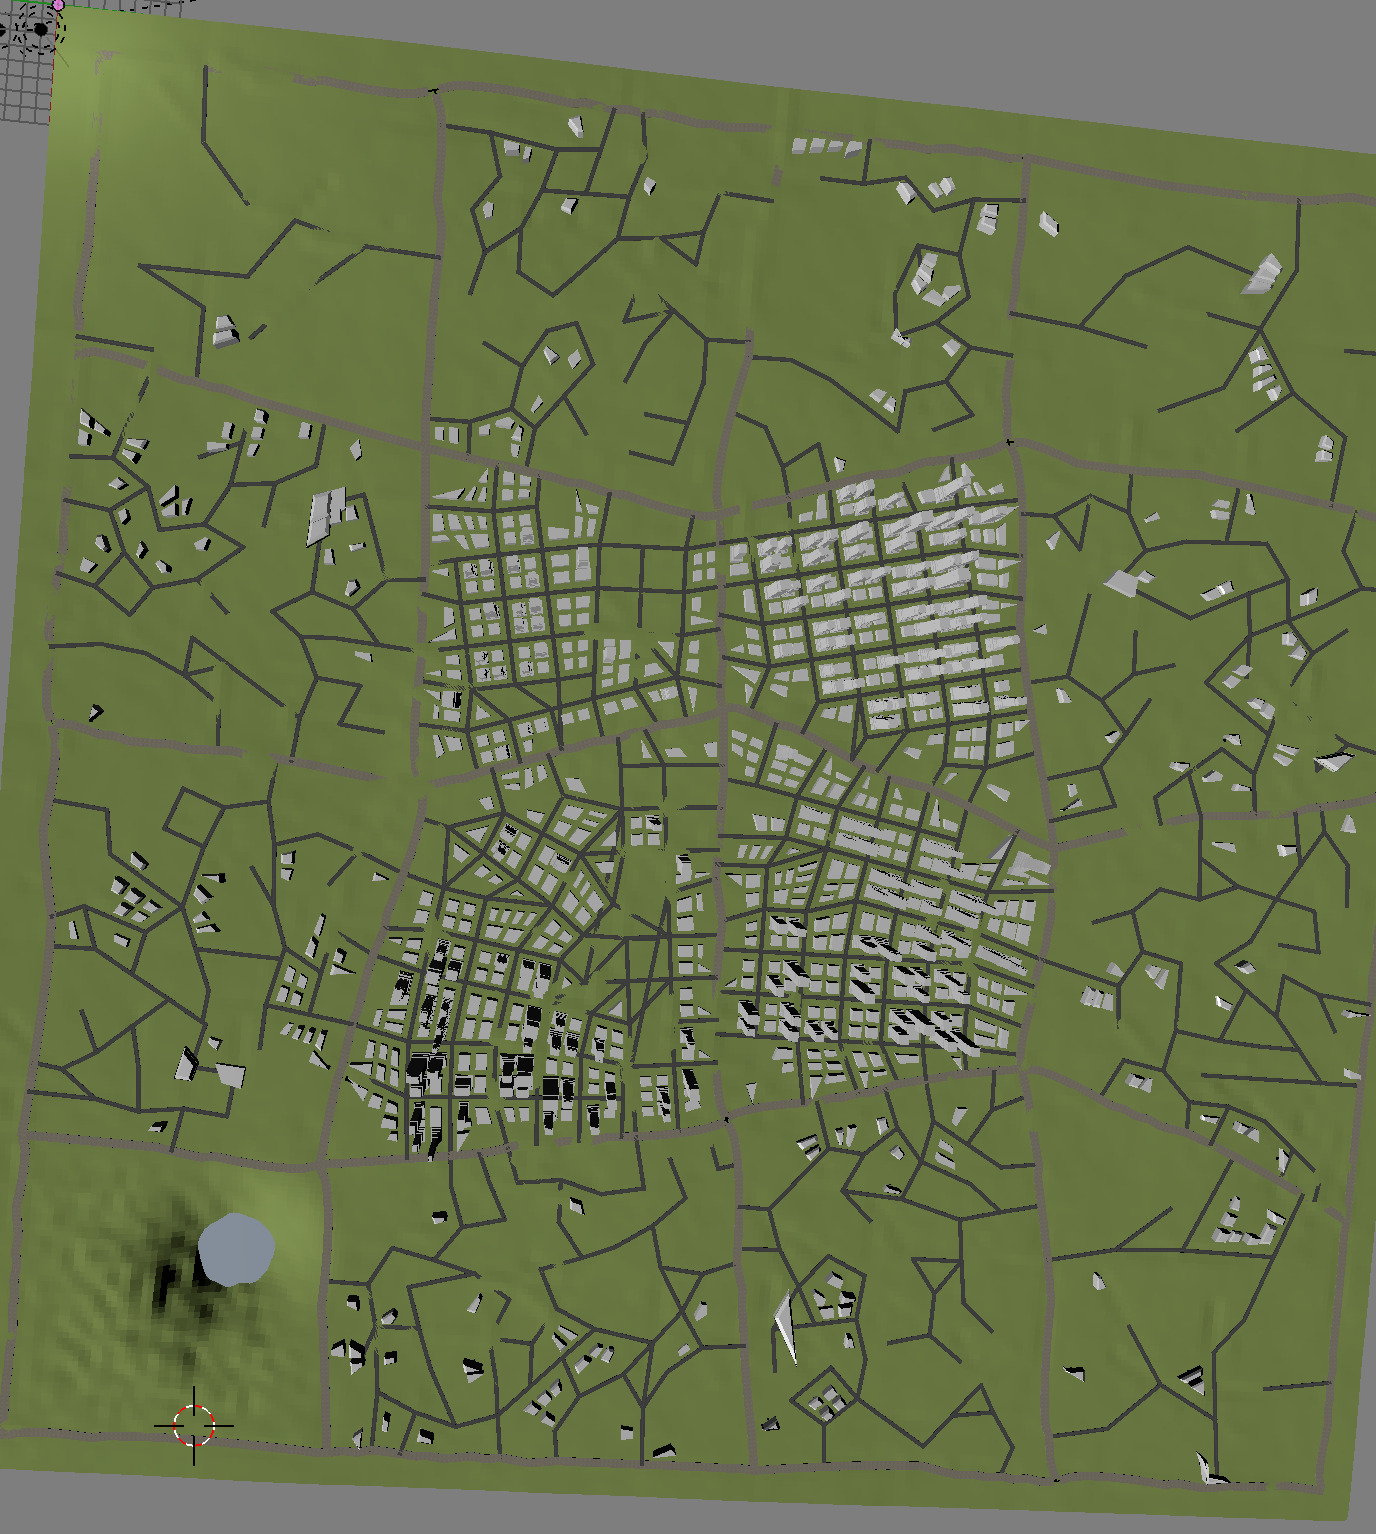
\includegraphics[width=\textwidth]{view3.png}



\bibliographystyle{authordate1}
\nocite{*}
\bibliography{../references/references.bib}



\end{document}